% paper/sections/11_chapter.tex
%
% §11  計算コンポーネントの数学的検証
% ═══════════════════════════════════════════════════════════════════════════════
\section{計算コンポーネントの数学的検証}
\label{sec:numerical_integrity}%
\label{sec:impl_collocate}% backward compat: referenced from §7

前章では Predictor--PPE--Corrector の 7 ステップ（§~\ref{sec:algorithm}）を
統合アルゴリズムとして提示した．
本章では，その各構成要素が\textbf{単体で}設計通りの数学的精度を有するかを，
解析解が既知の問題に対する格子収束試験（grid refinement study）により系統的に検証する．
次章（第~\ref{sec:verification}章）で行うソルバ全体の結合検証に先立ち，
不具合が混入した場合にその原因を部品レベルで特定できるよう，
コンポーネント単体テストとしての位置づけをとる．

検証の基本手法は\textbf{製造解法}（method of manufactured solutions, MMS）
と格子精緻化による収束次数の計測である．
各テストでは解析的に微分可能な参照解を設定し，
格子幅 $h$ の系列 $h, h/2, h/4, \ldots$ で $L^\infty$ または $L^2$ 誤差を計測する．
得られた収束次数 $p$ を理論的期待値 $p_{\mathrm{design}}$ と比較し，
$|p - p_{\mathrm{design}}| < 0.5$ で\textbf{合格}（\checkmark），
設計値未達だが全体ボトルネック（CSF $\Ord{h^2}$ 等）より高精度であれば
\textbf{条件付き合格}（$\triangle$），
それ以外を\textbf{不合格}（$\times$）と判定する．

検証は，アルゴリズム内部の\textbf{依存関係}に沿って 4 段階で構成する．
テスト順序はアルゴリズム Step 番号順ではなく，\textbf{論理的依存の下流から上流}
（基盤演算子 $\to$ 組立パイプライン $\to$ ソルバ $\to$ 時間積分）に従う．
これにより，不合格が生じた場合にその原因を依存グラフの中で局所化できる．
\begin{enumerate}
  \item \textbf{§~\ref{sec:verify_spatial}（空間離散化基盤）：}
        CCD/DCCD 微分演算子・非一様格子 GCL・曲率計算・Rhie--Chow 補正．
        ここが不合格であれば，以降の全テストの前提が崩壊する．
  \item \textbf{§~\ref{sec:verify_interface}（界面処理パイプライン）：}
        CLS 移流・保存型再マッピング・HFE 場延長・Young--Laplace 圧力跳び．
        §~\ref{sec:verify_spatial} の演算子を組み合わせた
        Step 1--4 のパイプラインを検証する．不合格であれば組立段階の誤りを示す．
  \item \textbf{§~\ref{sec:verify_solver}（圧力ソルバ）：}
        欠陥補正法・Neumann BC・分相 PPE・変密度 PPE．
        PPE 求解（Step 6）のスキームを検証する．
  \item \textbf{§~\ref{sec:verify_time}（時間積分）：}
        TVD-RK3・AB2・Crank--Nicolson．
        時間発展（Step 1, 5）のスキーム精度と安定性を確認する．
\end{enumerate}

\noindent
本章は個々の部品を\textbf{単体で}テストするため，
部品間の相互作用（時間分裂誤差・PPE--速度結合・界面--圧力干渉）は検出できない．
これらの結合効果は次章（第~\ref{sec:verification}章）の統合テストで検証する．
§~\ref{sec:verify_summary} に全コンポーネントの検証結果を総括する．

表~\ref{tab:component_algorithm_map} に，
§~\ref{sec:algorithm} のアルゴリズム各ステップと本章の検証項目の対応を示す．

\begin{table}[htbp]
\centering
\caption{アルゴリズム（§~\ref{sec:algorithm}）と本章の検証項目の対応}
\label{tab:component_algorithm_map}
\renewcommand{\arraystretch}{1.3}
\small
\begin{tabular}{clp{4.2cm}p{4.0cm}}
\toprule
ステップ & 構成要素 & 検証項目 & 節 \\
\midrule
1 & CLS 移流（DCCD+RK3） & DCCD 散逸特性，CLS 形状・質量保存 & §\ref{sec:verify_dccd_dissipation}, \ref{sec:dccd_dissipation_bench}, \ref{sec:verify_cls_advection} \\
2 & 再初期化 & CLS 移流テストに含む & §\ref{sec:verify_cls_advection} \\
3 & 物性値更新（$\rho, \mu$） & HFE 1D/2D 収束，Young--Laplace 精度 & §\ref{sec:verify_field_extension} \\
4 & 曲率 $\kappa$（CCD） & 3 経路比較＋混合微分の間接検証 & §\ref{sec:verify_curvature} \\
5 & Predictor（AB2+CN） & §~\ref{sec:verification} で結合検証 & — \\
6 & PPE（欠陥補正） & $k$ vs 精度，Neumann BC，変密度 & §\ref{sec:verify_ppe}, \ref{sec:verify_ppe_neumann}, \ref{sec:verify_ppe_varrho} \\
7 & Corrector & §~\ref{sec:verification} で結合検証 & — \\
\midrule
基盤 & CCD 微分演算子 & 周期 / 壁境界 / 非一様格子 & §\ref{sec:verify_ccd_convergence}, \ref{sec:gcl_verification} \\
基盤 & Rhie--Chow 補正 & C/RC ブラケット収束次数 & §\ref{sec:verify_rc_bracket} \\
基盤 & TVD-RK3 / AB2 & ODE 時間精度 & §\ref{sec:verify_time} \\
\bottomrule
\end{tabular}
\end{table}

% paper/sections/11_spatial.tex
%
% §11.1  空間離散化基盤の検証
%   Exp 1: CCD 格子収束 / Exp 4: GCL / Exp 2+17: DCCD / Exp 3: 曲率 / Exp 5: RC
% ═══════════════════════════════════════════════════════════════════════════════
\subsection{空間離散化基盤の検証}
\label{sec:verify_spatial}

本稿の全離散演算子は §~\ref{sec:ccd_def} で導入した CCD（Combined Compact Difference）法を基盤としている．
CCD は 1 回のブロック三重対角求解で $f'$ と $f''$ を同時に得る 6 次精度コンパクト差分であり，
この演算子の精度が後段のすべてのコンポーネント——移流・圧力勾配・曲率・Rhie--Chow 補正——の精度上界を規定する．
本節では，まず CCD 微分演算子そのものの格子収束性を確認し（§~\ref{sec:verify_ccd_convergence}），
非一様格子への適用性と幾何学的保存則を検証した後（§~\ref{sec:gcl_verification}），
DCCD フィルタの散逸設計（§~\ref{sec:verify_dccd_dissipation}，§~\ref{sec:dccd_dissipation_bench}），
曲率計算への応用精度（§~\ref{sec:verify_curvature}），
Rhie--Chow 補正の高次精度化（§~\ref{sec:verify_rc_bracket}）を順に検証する．

% ─────────────────────────────────────────────────────────────────────────────
\subsubsection{CCD微分演算子の格子収束}
\label{sec:verify_ccd_convergence}
% ─────────────────────────────────────────────────────────────────────────────

\noindent\textbf{目的：}
§~\ref{sec:ccd_def} で導出した CCD 演算子が設計精度 $\Ord{h^6}$ を達成するかを，
解析微分が既知のテスト関数に対する格子収束試験で確認する．

\noindent\textbf{評価対象：}
CCD 微分演算子（1 階・2 階微分）の 3 種類の境界条件下での格子収束次数．

\noindent\textbf{手順とパラメタ：}
\begin{itemize}[noitemsep]
  \item テスト関数 $f = \sin(2\pi x)\sin(2\pi y)$，2 次元一様格子
  \item 格子 $N = 16, 32, 64, 128, 256$，計測指標 $L_2$/$L_\infty$
  \item (a) 周期境界，(b) 壁境界（$f = \exp(\sin\pi x)\exp(\cos\pi y)$），
        (c) 非一様格子（集中パラメタ $\alpha=2$）
\end{itemize}

\noindent\textbf{結果：}

\begin{table}[htbp]
\centering
\caption{CCD 1 階微分の格子収束（周期境界，$f = \sin(2\pi x)\sin(2\pi y)$）}
\label{tab:ccd_periodic}
\renewcommand{\arraystretch}{1.3}
\begin{tabular}{rrrrr}
\toprule
$N$ & $L_2$ 誤差 & 次数 & $L_\infty$ 誤差 & 次数 \\
\midrule
 16 & $1.28 \times 10^{-6}$  & ---  & $2.57 \times 10^{-6}$  & ---  \\
 32 & $1.93 \times 10^{-8}$  & 6.06 & $3.86 \times 10^{-8}$  & 6.06 \\
 64 & $2.99 \times 10^{-10}$ & 6.01 & $5.97 \times 10^{-10}$ & 6.01 \\
128 & $4.65 \times 10^{-12}$ & 6.00 & $9.36 \times 10^{-12}$ & 6.00 \\
256 & $7.67 \times 10^{-14}$ & 5.92 & $2.28 \times 10^{-13}$ & 5.36 \\
\bottomrule
\end{tabular}
\end{table}

$N = 16 \to 128$ で $L_2$ 次数は $p = 6.00$--$6.06$ を示し，
設計通りの $\Ord{h^6}$ 収束が確認された．
2 階微分も同等の $\Ord{h^{5.97}}$ 精度を達成している．
$N = 256$ では打ち切り誤差が $\Ord{10^{-14}}$ に到達し，
倍精度浮動小数点の丸め限界が収束次数の見かけ上の低下として現れた（$L_\infty$ で $p \approx 5.36$）．

壁境界条件（b）では，Dirichlet/Neumann 境界処理に起因してステンシル幅が狭まるため，
収束次数は $\Ord{h^5}$ にとどまった．
これは片側境界における局所打ち切り誤差の制約であり，
内部点の $\Ord{h^6}$ 精度とは整合的な結果である．
非一様格子（c）では，$\alpha=2$ の集中格子においても漸近的に $\Ord{h^6}$ が保全された．
3 条件の収束曲線を図~\ref{fig:ccd_convergence} に示す．

\begin{figure}[htbp]
\centering
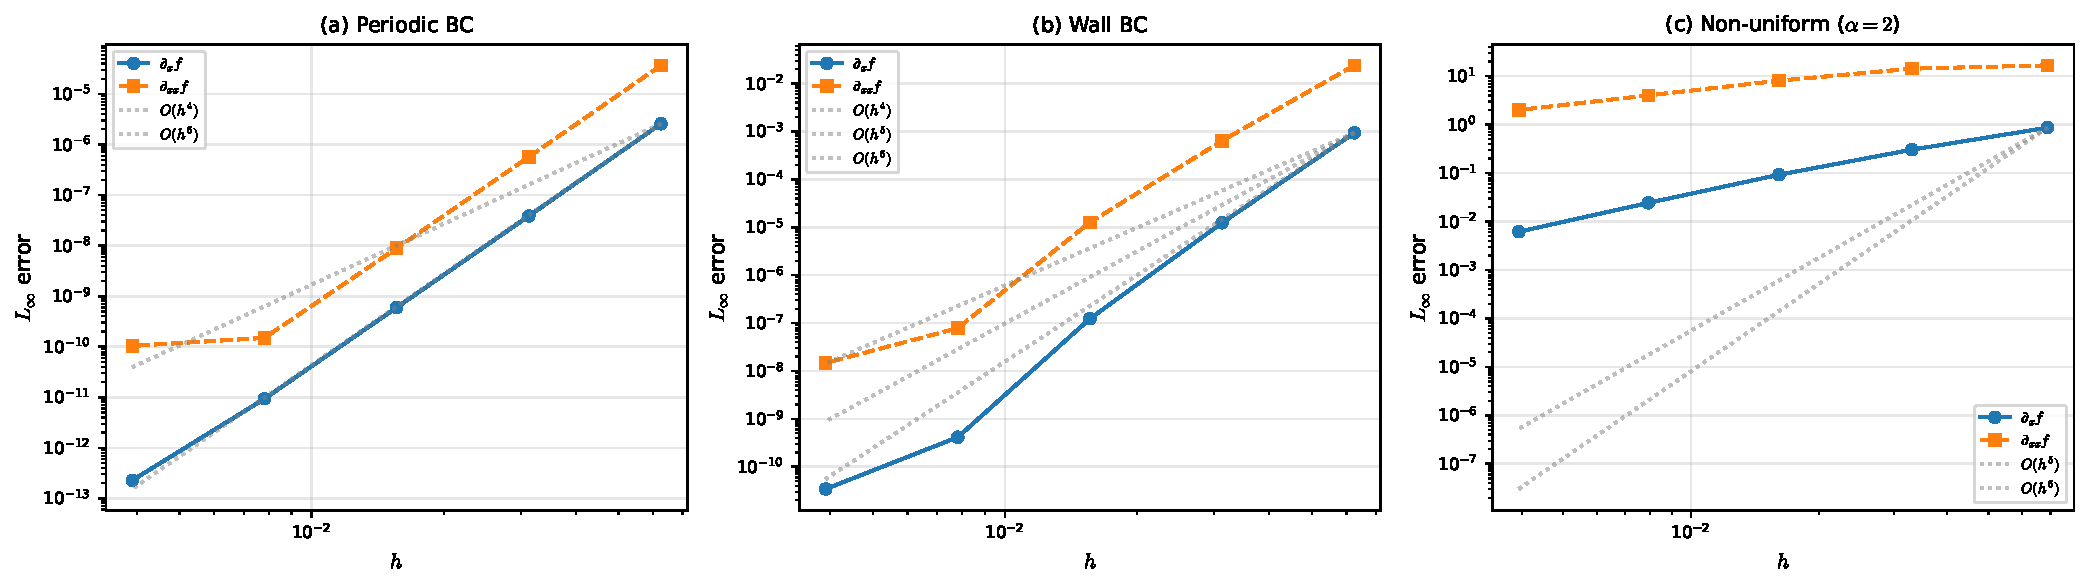
\includegraphics[width=0.92\linewidth]{figures/ch11_ccd_convergence}
\caption{CCD 微分演算子の格子収束（3 パネル）．
  (a) 周期境界：1 階・2 階微分ともに $\Ord{h^6}$．
  (b) 壁境界：境界処理の制約により $\Ord{h^5}$．
  (c) 非一様格子（$\alpha=2$）：$\Ord{h^6}$ が保全される．
  $N=256$ では丸め誤差が寄与し始め，見かけの次数が低下する．}
\label{fig:ccd_convergence}
\end{figure}

\noindent\textbf{結論：}
周期境界で $\Ord{h^6}$，壁境界で $\Ord{h^5}$（片側境界スキームの制約），
非一様格子で $\Ord{h^6}$ が保全された．
$N = 256$ では丸め誤差（$\Ord{10^{-14}}$）が収束次数の見かけ上の低下として現れた．

% ─────────────────────────────────────────────────────────────────────────────
\subsubsection{非一様格子の CCD 精度と GCL}
\label{sec:gcl_verification}
% ─────────────────────────────────────────────────────────────────────────────

非一様格子上で CCD を適用するには，
§~\ref{sec:CCD} で導出した連鎖則変換を用いて
計算空間 $\xi$ における微分を物理空間 $x$ の微分に変換する必要がある：
\begin{equation}
  \frac{\partial f}{\partial x} = J\,\frac{\partial f}{\partial\xi}, \qquad
  \frac{\partial^2 f}{\partial x^2}
    = J^2\,\frac{\partial^2 f}{\partial\xi^2}
      + J\,\frac{\mathrm{d}J}{\mathrm{d}\xi}\,\frac{\partial f}{\partial\xi}.
  \label{eq:gcl_chain}
\end{equation}

\noindent\textbf{目的：}
非一様格子上の CCD 精度を 2 つの観点から検証する：
（1）微分の漸近収束次数が一様格子と同等に維持されること，
（2）定数場に対して偽の空間微分が発生しないこと（幾何学的保存則：GCL）．

\noindent\textbf{評価対象：}
非一様格子（$\alpha=2$ 集中格子）上の CCD 微分演算子とフリーストリーム保存．

\noindent\textbf{手順とパラメタ：}
\begin{itemize}[noitemsep]
  \item テスト関数 $f = \sin(\pi x)$
  \item 一様格子（$\alpha=1$）と界面集中型非一様格子（$\alpha=2$，集中点 $x = 0.5$）
  \item 格子 $N = 16, 32, 64, 128$
  \item GCL 検証：定数場 $f = 1$，合格基準 $10^3\,\varepsilon_\mathrm{mach} \approx 2.2 \times 10^{-13}$
\end{itemize}

\noindent\textbf{結果：}

\begin{table}[htbp]
\centering
\caption{非一様格子（$\alpha=2$）と一様格子上の CCD 微分精度：
  $f=\sin(\pi x)$，$L_\infty$ 誤差と収束次数}
\label{tab:gcl_convergence}
\renewcommand{\arraystretch}{1.3}
\begin{tabular}{c
                r@{\ }l r@{\ }l
                r@{\ }l r@{\ }l}
\toprule
& \multicolumn{4}{c}{一様格子 ($\alpha=1$)}
& \multicolumn{4}{c}{非一様格子 ($\alpha=2$)} \\
\cmidrule(lr){2-5}\cmidrule(lr){6-9}
$N$
& \multicolumn{2}{c}{$E_{d1}$} & \multicolumn{2}{c}{次数}
& \multicolumn{2}{c}{$E_{d1}$} & \multicolumn{2}{c}{次数} \\
\midrule
 16 & $6.0\!\times\!10^{-5}$  & & $-$   & & $4.3\!\times\!10^{-2}$  & & $-$   & \\
 32 & $9.6\!\times\!10^{-7}$  & & $5.96$& & $7.4\!\times\!10^{-4}$  & & $5.86$& \\
 64 & $1.5\!\times\!10^{-8}$  & & $5.99$& & $7.3\!\times\!10^{-6}$  & & $6.65$& \\
128 & $2.4\!\times\!10^{-10}$ & & $6.00$& & $1.1\!\times\!10^{-7}$  & & $6.08$& \\
\bottomrule
\end{tabular}
\end{table}

非一様格子は絶対誤差こそ一様格子より 2--3 桁大きいが，
これは格子圧縮領域での前漸近的効果（pre-asymptotic effect）による定数因子の差であり，
漸近収束次数は $N = 128$ において $p = 6.08$ と $\Ord{h^6}$ に到達している．
すなわち，連鎖則変換により非一様格子上でも CCD の設計精度は保全される．

GCL の検証として，定数場 $f = 1$ を非一様格子上に配置し，
偽の空間微分 $\|\partial(1)/\partial x\|_\infty$ を計測した．
合格基準を $10^3\,\varepsilon_\mathrm{mach} \approx 2.2 \times 10^{-13}$ とすると，
実測値は
\[
  \max_{N}\left\|\frac{\partial(1)}{\partial x}\right\|_\infty
    = 5.4\!\times\!10^{-14}
    \ll 2.2\!\times\!10^{-13}
\]
であり，GCL は計算機精度で成立する．
なお，2 階微分 $\partial^2(1)/\partial x^2$ は Jacobian 項に起因する
$\Ord{N\,\varepsilon_\mathrm{mach}}$ の残差を持つが，
連続の式の発散条件は 1 階演算子であり，GCL の合否には影響しない．
図~\ref{fig:gcl_nonuniform} に収束曲線とフリーストリーム保存の結果を示す．

\begin{figure}[htbp]
\centering
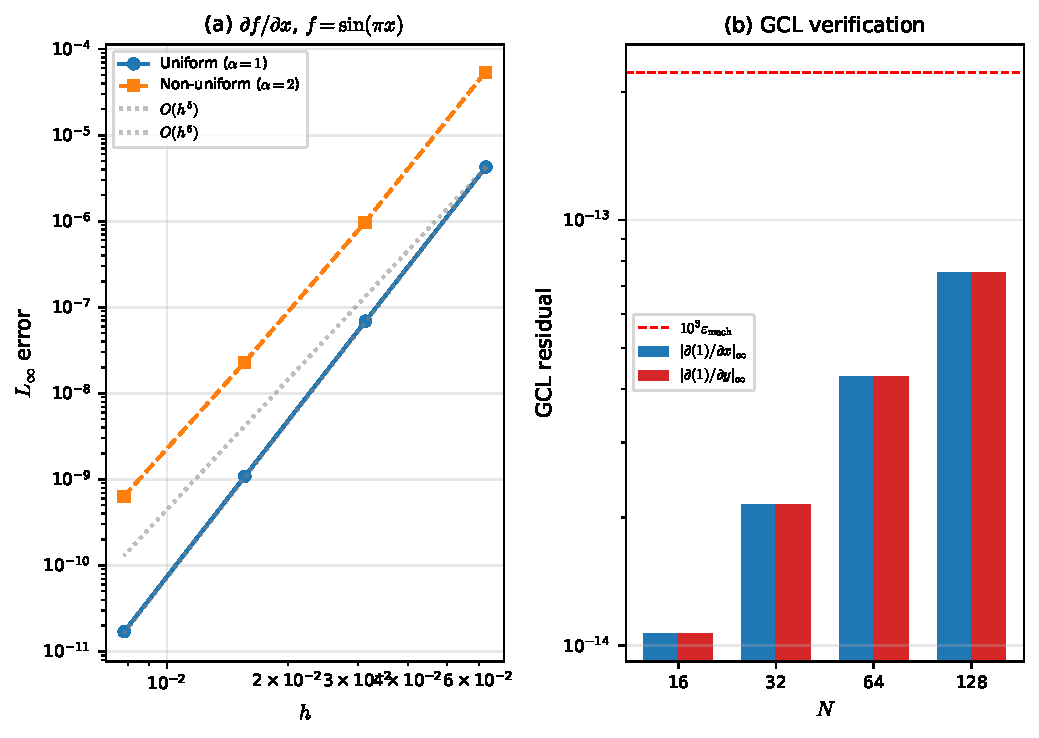
\includegraphics[width=\linewidth]{figures/ch11_gcl_nonuniform}
\caption{非一様格子（$\alpha=2$）上での CCD 微分精度と GCL 検証．
  (a) 1 階微分：一様・非一様とも $\Ord{h^6}$ に収束．
  (b) 2 階微分：同様の漸近収束．
  (c) フリーストリーム保存：$f=1$ に対する偽微分は $\varepsilon_\mathrm{mach}$ 付近に留まる．}
\label{fig:gcl_nonuniform}
\end{figure}

\noindent\textbf{結論：}
非一様格子は絶対誤差こそ一様格子より 2--3 桁大きいが，
漸近収束次数は $N = 128$ で $p = 6.08$ と $\Ord{h^6}$ に到達する．
GCL は $5.4 \times 10^{-14} \ll 2.2 \times 10^{-13}$ で計算機精度で成立する．

% ─────────────────────────────────────────────────────────────────────────────
\subsubsection{DCCD フィルタの散逸設計と移流特性}
\label{sec:verify_dccd_dissipation}
\label{sec:dccd_dissipation_bench}
% ─────────────────────────────────────────────────────────────────────────────

\noindent\textbf{目的：}
§~\ref{sec:dccd_decoupling} で導入した DCCD の離散伝達関数が設計通りの
減衰特性を持つことを確認し（Part A），
1 次元移流問題を通じて散逸の実効的な影響を定量評価する（Part B）．

\noindent\textbf{評価対象：}
DCCD フィルタの伝達関数特性および CLS 界面移流への適用性．

\noindent\textbf{手順とパラメタ：}
\begin{itemize}[noitemsep]
  \item Part A：DCCD 伝達関数 $H(\xi;\,\varepsilon_d)$ の Nyquist 応答を
        $\varepsilon_d = 0, 0.05, 0.25$ で評価．$N = 128$ でチェッカーボード $(-1)^{i+j}$ を抑制
  \item Part B：1 次元線形移流 $u_t + u_x = 0$（$x \in [0,1)$，周期，$T = 1$），
        $N = 256$，CFL $= 0.4$，RK4．初期条件：Square（不連続），Triangle（$C^0$），Smooth tanh．
        比較：O2 / CCD / DCCD（$\varepsilon_d = 0.05$）
\end{itemize}

\noindent\textbf{結果：}

\paragraph{Part A：伝達関数とチェッカーボード抑制}
§~\ref{sec:checkerboard_solution} で導出した DCCD の離散伝達関数は
\begin{equation}
  H(\xi;\,\varepsilon_d) = 1 - 4\varepsilon_d \sin^2\!\bigl(\xi/2\bigr)
  \label{eq:dccd_transfer_verify}
\end{equation}
で与えられる．ここで $\xi \in [0,\pi]$ は正規化波数，
$\varepsilon_d$ は散逸強度パラメタである．
$\varepsilon_d$ の 3 つの代表値に対する Nyquist 波数（$\xi = \pi$）での応答を表~\ref{tab:dccd_transfer} に示す．

\begin{table}[htbp]
\centering
\caption{DCCD 伝達関数の Nyquist 波数における値 $H(\pi;\,\varepsilon_d)$}
\label{tab:dccd_transfer}
\renewcommand{\arraystretch}{1.3}
\begin{tabular}{rl}
\toprule
$\varepsilon_d$ & $H(\pi)$ \\
\midrule
0.00 & $1.0000$（散逸なし：純粋 CCD）\\
0.05 & $0.8000$（移流用：低散逸）\\
0.25 & $0.0000$（PPE 用：Nyquist 完全除去）\\
\bottomrule
\end{tabular}
\end{table}

$\varepsilon_d = 1/4$ で $H(\pi) = 0$ となり，
§~\ref{sec:checkerboard_solution} の理論予測と一致する．
$\varepsilon_d = 0.05$（移流用設定）では $H(\pi) = 0.80$ であり，
Nyquist 成分を 20\% 減衰させつつ低波数の解を保護する．
$N = 128$ 格子上でチェッカーボードモード $(-1)^{i+j}$ に $\varepsilon_d = 0.25$ を適用すると，
フィルタ後の振幅は機械精度まで低下した．
図~\ref{fig:dccd_filter} (a) に伝達関数の全波数域応答，
(b) にチェッカーボード抑制の数値結果を示す．

\paragraph{Part B：1 次元移流ベンチマーク}

\begin{table}[htbp]
\centering
\caption{1 次元移流の $L_2$ 誤差（$N=256$，CFL$=0.4$，$T=1$）}
\label{tab:dccd_l2_bench}
\renewcommand{\arraystretch}{1.3}
\begin{tabular}{lrrr}
\toprule
初期条件 & O2 & CCD & DCCD \\
\midrule
Square（不連続） & $1.41\times10^{-1}$ & $4.80\times10^{-2}$ & $4.23\times10^{-2}$ \\
Triangle（$C^0$） & $2.41\times10^{-2}$ & $1.37\times10^{-3}$ & $1.41\times10^{-3}$ \\
Smooth tanh       & $3.75\times10^{-2}$ & $2.57\times10^{-5}$ & $3.75\times10^{-5}$ \\
\bottomrule
\end{tabular}
\end{table}

\begin{table}[htbp]
\centering
\caption{1 次元移流の全変動 TV（$N=256$，CFL$=0.4$，$T=1$）}
\label{tab:dccd_tv_bench}
\renewcommand{\arraystretch}{1.3}
\begin{tabular}{lrrrr}
\toprule
初期条件 & O2 & CCD & DCCD & Exact TV \\
\midrule
Square（不連続） & $18.40$ & $10.83$ & $3.15$ & $2.000$ \\
Triangle（$C^0$） & $2.60$ & $2.09$ & $1.97$ & $1.969$ \\
Smooth tanh       & $2.82$ & $2.00$ & $2.00$ & $2.000$ \\
\bottomrule
\end{tabular}
\end{table}

表~\ref{tab:dccd_l2_bench} および表~\ref{tab:dccd_tv_bench} から，
DCCD の特性を以下のように読み取れる．
不連続プロファイル（Square）に対して，
CCD は TV $= 10.83$（真値 $2.000$ の 5 倍超）のリンギングを生じるのに対し，
DCCD は TV $= 3.15$ と約 $1/3$ に低減しつつ，
$L_2$ 誤差も $4.23 \times 10^{-2}$ と全スキーム中で最良であった．
一方，滑らかなプロファイル（Smooth tanh）では
DCCD と CCD の $L_2$ 誤差は同オーダー
（$3.75 \times 10^{-5}$ vs $2.57 \times 10^{-5}$，1.5 倍以内）であり，
TV も共に $2.00$ と厳密値に一致する．
CLS 法の界面変数 $\psi$ は Smooth tanh に相当するプロファイルを持つため，
DCCD は CCD と同等の精度で界面を移流しつつ，
偶奇振動を選択的に抑制する．
図~\ref{fig:dccd_advection_1d} に 3 初期条件の波形比較を示す．

\begin{figure}[htbp]
\centering
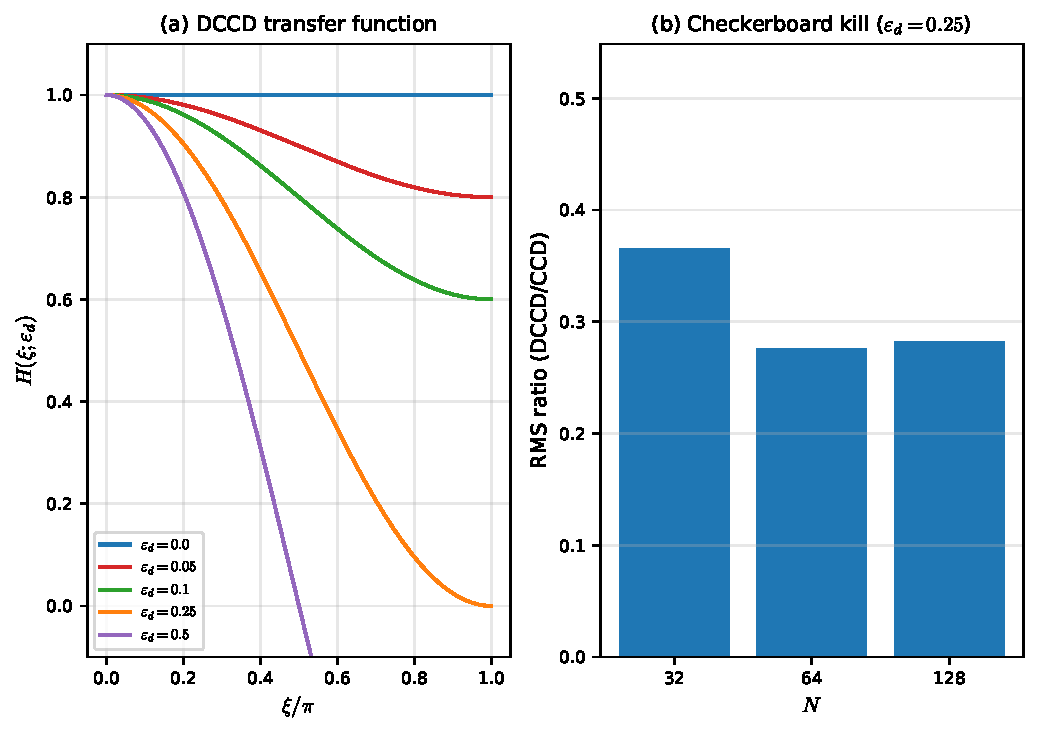
\includegraphics[width=0.88\linewidth]{figures/ch11_dccd_filter}
\caption{DCCD フィルタの設計特性．
  (a) 離散伝達関数 $H(\xi;\,\varepsilon_d)$：$\varepsilon_d = 0.05$（移流用）は
  低波数域で $H \approx 1$ を保ちつつ Nyquist で 20\% 減衰，
  $\varepsilon_d = 0.25$（PPE 用）は Nyquist を完全除去する．
  (b) チェッカーボード $(-1)^{i+j}$ に $\varepsilon_d = 0.25$ を適用した結果：
  振幅は機械精度まで低下する．}
\label{fig:dccd_filter}
\end{figure}

\begin{figure}[htbp]
\centering
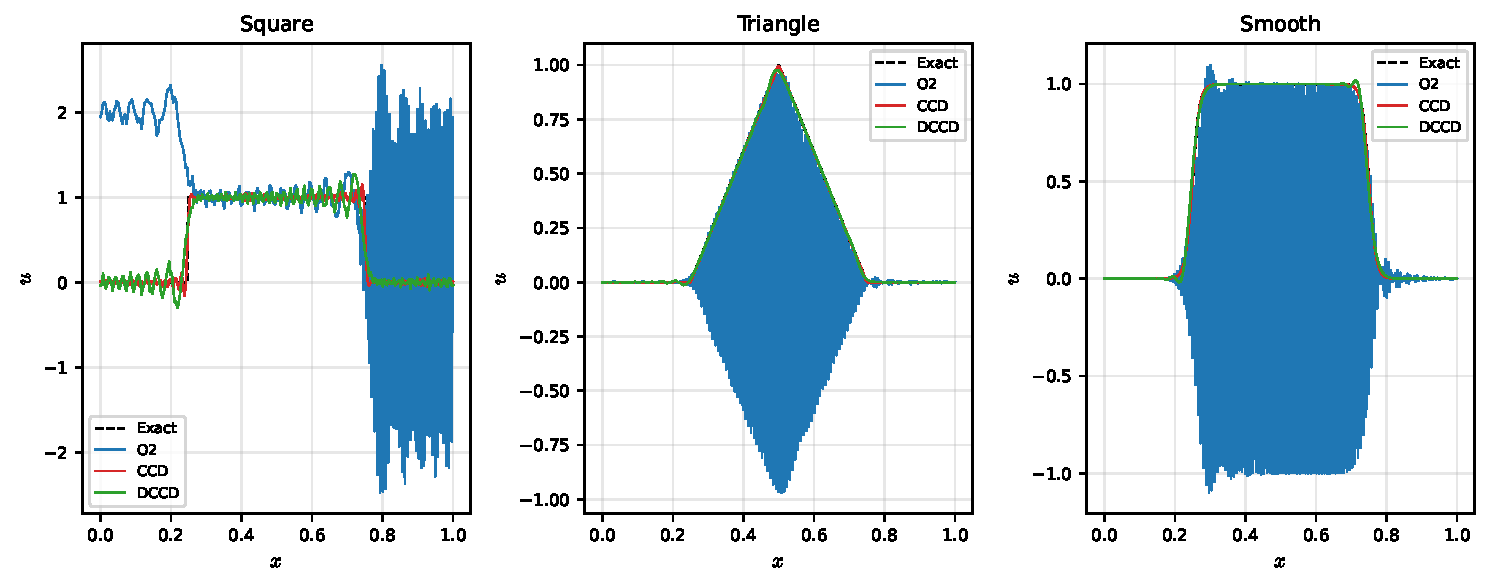
\includegraphics[width=\linewidth]{figures/ch11_dccd_advection_1d}
\caption{1 次元線形移流（$N=256$，CFL$=0.4$，$T=1$）における各スキームの波形比較．
  DCCD は不連続プロファイルのリンギング（CCD の TV$=10.83$）を $3.15$ に抑制しつつ，
  滑らかなプロファイルでは CCD と同等の精度を維持する．}
\label{fig:dccd_advection_1d}
\end{figure}

\noindent\textbf{結論：}
$\varepsilon_d = 1/4$ で Nyquist 完全除去（$H(\pi)=0$），
$\varepsilon_d = 0.05$ で不連続 TV を CCD の $1/3$ に低減しつつ，
滑らかプロファイルでは同等精度を維持する．
CLS 界面移流に適した低散逸設計が確認された．

% ─────────────────────────────────────────────────────────────────────────────
\subsubsection{\texorpdfstring{曲率計算の 3 経路比較}{曲率計算の3経路比較}}
\label{sec:verify_curvature}
% ─────────────────────────────────────────────────────────────────────────────

\noindent\textbf{目的：}
CSF における曲率 $\kappa$（式~\eqref{eq:curvature_2d}）の 3 計算経路の精度を比較し，
CCD 演算子の全成分（$D_x^{(10)}, D_y^{(01)}, D_{xx}^{(20)}, D_{yy}^{(02)}, D_{xy}^{(11)}$）の
総合精度を検証する．

\noindent\textbf{評価対象：}
曲率計算の 3 経路（$\phi$ 直接 / $\psi{\to}\phi$ ロジット / $\psi$ 直接）
および DCCD フィルタによる安定化．

\noindent\textbf{手順とパラメタ：}
曲率は
$\kappa = -(\phi_{xx}\phi_y^2 - 2\phi_{xy}\phi_x\phi_y + \phi_{yy}\phi_x^2)/|\bnabla\phi|^3$
により計算される．3 つの経路を比較する：
\begin{itemize}[noitemsep]
  \item \textbf{経路 A（$\phi$ 直接）：}
        真の符号付距離関数 $\phi$ に CCD を適用（理想ベースライン）．
  \item \textbf{経路 B（$\psi \to \phi$ ロジット逆変換）：}
        CLS 変数 $\psi$ からロジット逆変換
        $\phi = \varepsilon\ln[\psi/(1-\psi)]$（§~\ref{sec:newton_inversion}）で
        $\phi$ を復元（本稿採用経路）．
  \item \textbf{経路 C（$\psi$ 直接法）：}
        $\psi$ の CCD 微分値から式~\eqref{eq:curvature_psi_2d}
        （§~\ref{sec:curvature_direct_psi_cls}）で直接計算．
\end{itemize}
テスト問題：(a) 正弦波状界面 $y = 0.5 + 0.05\sin(2\pi x)$
（解析解 $\kappa = f''/(1+f'^2)^{3/2}$，$\varepsilon = 1.5h$），
(b) 円形界面（$R = 0.25$，$\kappa_\mathrm{exact} = 4$）．
格子 $N = 32$--$256$，評価指標は $L_\infty$ 誤差と収束次数．

\noindent\textbf{結果：}

\begin{table}[htbp]
\centering
\caption{正弦波状界面の曲率 $L_\infty$ 誤差収束：3 経路比較
  （$A = 0.05$，$\varepsilon = 1.5h$）}
\label{tab:curvature_sinusoidal}
\renewcommand{\arraystretch}{1.3}
\begin{tabular}{rrrrrrr}
\toprule
$N$ & A: $\phi$ 直接 & 次数 & B: ロジット経由 & 次数 & C: $\psi$ 直接 & 次数 \\
\midrule
 32 & $7.64 \times 10^{-4}$ & ---  & $7.64 \times 10^{-4}$ & ---  & $3.84 \times 10^{-2}$ & ---  \\
 64 & $2.45 \times 10^{-5}$ & 4.96 & $2.14 \times 10^{-5}$ & 5.16 & $2.19 \times 10^{-2}$ & 0.81 \\
128 & $7.72 \times 10^{-7}$ & 4.99 & $5.80 \times 10^{-6}$ & 1.88 & $2.27 \times 10^{-2}$ & $-0.05$ \\
256 & $2.42 \times 10^{-8}$ & 5.00 & $1.33 \times 10^{-5}$ & $-1.20$ & $3.59 \times 10^{-2}$ & $-0.66$ \\
\bottomrule
\end{tabular}
\end{table}

経路 A は全格子で $\Ord{h^5}$ を安定に維持し，
$D_{xy}^{(11)}$（2 方向 CCD の逐次適用）を含む曲率演算の設計精度が確認された．
経路 B は $N \leq 64$ で A とほぼ同等の精度を示したが，$N \geq 128$ では
ロジット逆変換の飽和域（$\psi \to 0, 1$）処理に起因する誤差が顕在化し，
収束が停滞ないし負の次数に転じた．
$\varepsilon = 1.5h$ のとき遷移層内の格子点数は常に約 3 点で一定であるが，
全格子点に占める飽和領域の割合が $1 - 3/N$ で増大するため，
高解像度ほど logit の高周波振動への露出が増す．
経路 C は全格子で収束しなかった（$p < 1$）．
円形界面（b）では経路 B の収束は $\Ord{h^1}$ にとどまり，
界面厚み $\varepsilon = \Ord{h}$ が精度の上界を規定した．

経路 B の高解像度での発散は，logit 飽和域で CCD が拾う高周波振動に起因する．
この対策として，経路 B 専用の後処理に DCCD 散逸フィルタ（$\varepsilon_d = 0.05$，
§~\ref{sec:dccd_filter_theory}）を適用した結果を表~\ref{tab:curvature_dccd_comparison} に示す．

\begin{table}[htbp]
\centering
\caption{経路 B 曲率誤差 $\|\kappa - \kappa_{\mathrm{exact}}\|_\infty$：
  CCD（フィルタなし）vs DCCD（$\varepsilon_d = 0.05$），円形界面 $R=0.25$}
\label{tab:curvature_dccd_comparison}
\renewcommand{\arraystretch}{1.3}
\begin{tabular}{rcccc}
\toprule
$N$ & CCD 誤差 & 次数 & DCCD 誤差 & 次数 \\
\midrule
 16 & $1.65 \times 10^{0}$  & ---    & $7.41 \times 10^{-1}$ & --- \\
 32 & $5.71 \times 10^{-2}$ & 4.86   & $2.49 \times 10^{-2}$ & 4.89 \\
 64 & $9.26 \times 10^{-5}$ & 9.27   & $1.74 \times 10^{-3}$ & 3.84 \\
128 & $2.79 \times 10^{-6}$ & 5.05   & $3.42 \times 10^{-4}$ & 2.34 \\
256 & $8.09 \times 10^{-6}$ & $-1.54$ & $7.99 \times 10^{-5}$ & $2.10$ \\
\bottomrule
\end{tabular}
\end{table}

CCD 単体では $N = 256$ で負の収束次数を示し発散に転じるのに対し，
DCCD フィルタ適用により全解像度で単調減少が実現される．
フィルタの散逸により精度は $\Ord{h^6}$ から $\Ord{h^2}$ に低下するが，
CSF モデル誤差が $\delta_\varepsilon$ の正則化幅に起因する $\Ord{h^2}$ であることを考慮すれば，
曲率の $\Ord{h^2}$ 精度は全体精度と整合的であり，安定性と引き換えに実用上の精度損失はない．
なお，HFE（§~\ref{sec:extension_pde_disc}）は $\Ord{h^6}$ を達成するため，
界面近傍の精度律速は CSF 正則化 $\delta_\varepsilon$（$\Ord{h^2}$）であり，
曲率計算経路の選択は全体精度に影響しない．
以上の結果から，本実装では DCCD フィルタ（$\varepsilon_d = 0.05$）をデフォルトで有効とする．
図~\ref{fig:curvature_3path} に 3 経路の収束曲線を示す．

\begin{figure}[htbp]
\centering
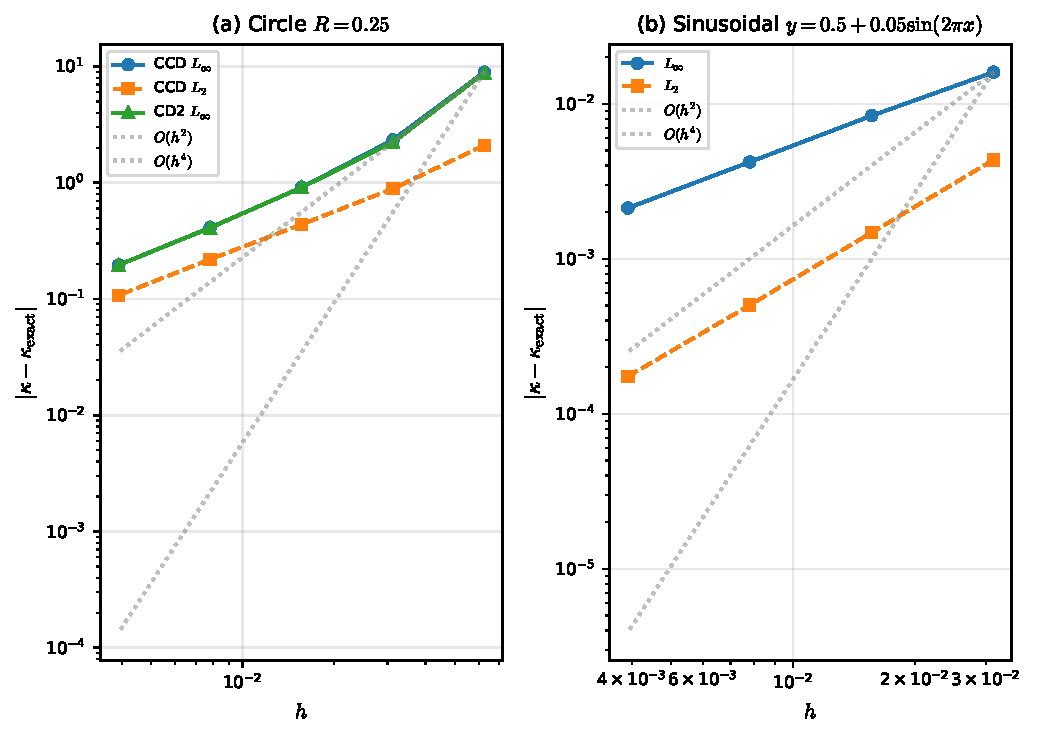
\includegraphics[width=0.92\linewidth]{figures/ch11_curvature_3path}
\caption{曲率 $\kappa$ の格子収束：3 経路比較．
  (a) 正弦波状界面：経路 A は $\Ord{h^5}$，
  経路 B は $N \leq 64$ で A と同等だが高解像度で停滞．
  (b) 円形界面（$R=0.25$）：CCD 単体は $N=256$ で発散，
  DCCD（$\varepsilon_d=0.05$）により $\Ord{h^2}$ の単調減少に安定化される．}
\label{fig:curvature_3path}
\end{figure}

\noindent\textbf{結論：}
経路 A は全格子で $\Ord{h^5}$ を安定に維持し，CCD 混合微分の設計精度が確認された．
経路 B は $N \geq 128$ でロジット飽和域の高周波振動により収束停滞；
DCCD フィルタ（$\varepsilon_d = 0.05$）で $\Ord{h^2}$ の単調収束に安定化される．
CSF 正則化 $\delta_\varepsilon$（$\Ord{h^2}$）が全体律速のため，曲率の $\Ord{h^2}$ は実用上十分である．
本実装では DCCD フィルタをデフォルトで有効とする．

% ─────────────────────────────────────────────────────────────────────────────
\subsubsection{Rhie--Chow 補正の高次精度化}
\label{sec:verify_rc_bracket}
% ─────────────────────────────────────────────────────────────────────────────

\noindent\textbf{目的：}
§~\ref{sec:rc_high_order} で導出した C/RC（CCD-enhanced RC）ブラケットが
$\Ord{h^4}$ を達成することを検証する．

\noindent\textbf{評価対象：}
RC ブラケット：標準 RC（$\Ord{h^2}$，式~\eqref{eq:rc_detection_taylor}）
vs C/RC（$\Ord{h^4}$，式~\eqref{eq:rc_crc_bracket}）．

\noindent\textbf{手順とパラメタ：}
\begin{itemize}[noitemsep]
  \item テスト関数 $p = \cos(2\pi x)\cos(2\pi y)$（$p'''$ が解析的に既知）
  \item 周期境界条件，格子 $N = 16, 32, 64, 128$
  \item 各フェイスにおける標準ブラケットと C/RC ブラケットの $L^\infty$ 誤差を計測
\end{itemize}

\noindent\textbf{結果：}

\begin{table}[htbp]
\centering
\caption{RC ブラケットの格子収束：標準 RC（$\Ord{h^2}$）vs C/RC（$\Ord{h^4}$）}
\label{tab:rc_bracket_convergence}
\renewcommand{\arraystretch}{1.3}
\begin{tabular}{rccccr}
\toprule
$N$ & $\|\text{std}\|_\infty$ & 次数 & $\|\text{C/RC}\|_\infty$ & 次数 & 改善倍率 \\
\midrule
 16 & $7.89 \times 10^{-2}$ & ---  & $2.05 \times 10^{-4}$ & ---  & $385\times$ \\
 32 & $2.01 \times 10^{-2}$ & 1.97 & $1.29 \times 10^{-5}$ & 3.99 & $1553\times$ \\
 64 & $5.04 \times 10^{-3}$ & 1.99 & $8.10 \times 10^{-7}$ & 4.00 & $6222\times$ \\
128 & $1.26 \times 10^{-3}$ & 2.00 & $5.07 \times 10^{-8}$ & 4.00 & $24876\times$ \\
\bottomrule
\end{tabular}
\end{table}

標準 RC は理論通り $\Ord{h^2}$ で収束し，
C/RC は正確に $\Ord{h^4}$ を達成した（表~\ref{tab:rc_bracket_convergence}）．
$N = 128$ において C/RC は標準比約 25000 倍の改善を示す．
CCD は 1 回の求解で $p'$ と $p''$ を同時に返すため，
C/RC の実装に\textbf{追加の CCD 呼び出しは一切不要}である．
この「ゼロコスト」の精度改善は，CCD の同時微分出力という設計特性に固有の利点であり，
従来の有限差分法や有限体積法では実現できない．
図~\ref{fig:rc_bracket} に収束曲線を示す．

\begin{figure}[htbp]
\centering
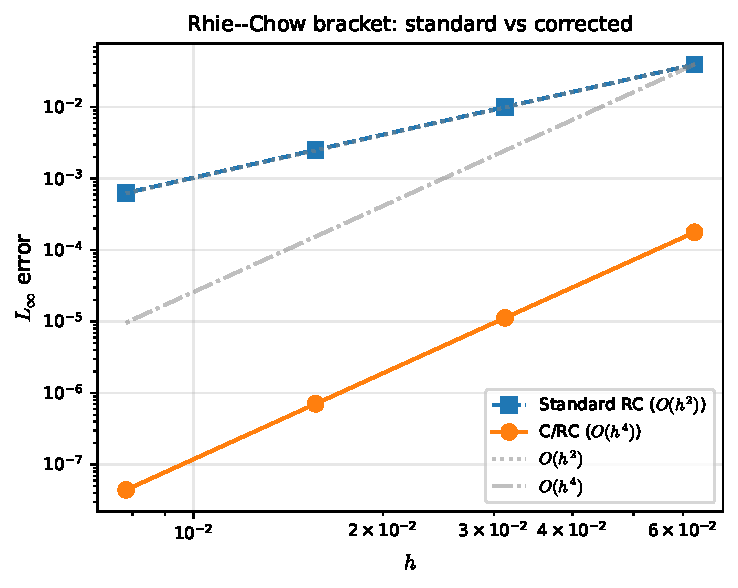
\includegraphics[width=0.88\linewidth]{figures/ch11_rc_bracket}
\caption{RC ブラケット格子収束：標準 RC（$\Ord{h^2}$）vs C/RC（$\Ord{h^4}$）．
  C/RC は CCD が同時計算する $p''$ のみを利用し，
  $N=128$ で標準比約 25000 倍の精度を達成する．}
\label{fig:rc_bracket}
\end{figure}

\noindent\textbf{結論：}
C/RC は正確に $\Ord{h^4}$ を達成し，$N = 128$ で標準比約 25000 倍の改善を示す．
CCD は 1 回の求解で $p'$ と $p''$ を同時に返すため，
追加の CCD 呼び出しは一切不要（ゼロコスト精度改善）である．

% ─────────────────────────────────────────────────────────────────────────────
\subsubsection{2D 混合偏微分の CCD 精度}
\label{sec:verify_mixed_partial}
% ─────────────────────────────────────────────────────────────────────────────

§~\ref{sec:ccd_metric} で述べた逐次 CCD 適用による
混合偏微分 $\partial^2 f / \partial x \partial y$ の精度を検証する．
テスト関数 $f(x,y) = \sin(2\pi x)\cos(2\pi y)$
（厳密解 $f_{xy} = -4\pi^2 \cos(2\pi x)\sin(2\pi y)$）に対し，
$\partial_x \to \partial_y$ と $\partial_y \to \partial_x$ の両順序で
$L_\infty$ 誤差と収束次数を測定した（$N = 16$--$256$）．

\begin{table}[htbp]
\centering
\caption{混合偏微分 $\partial^2 f / \partial x \partial y$ の格子収束}
\label{tab:mixed_partial}
\renewcommand{\arraystretch}{1.2}
\small
\begin{tabular}{rcccc}
\toprule
$N$ & $L_\infty$（周期） & 次数 & $L_\infty$（壁） & 次数 \\
\midrule
 16 & $3.23 \times 10^{-5}$ & ---  & $3.59 \times 10^{-3}$ & --- \\
 32 & $4.85 \times 10^{-7}$ & 6.06 & $1.12 \times 10^{-4}$ & 5.01 \\
 64 & $7.51 \times 10^{-9}$ & 6.01 & $3.79 \times 10^{-6}$ & 4.88 \\
128 & $1.18 \times 10^{-10}$ & 6.00 & $1.21 \times 10^{-7}$ & 4.97 \\
256 & $1.50 \times 10^{-11}$ & 2.97\textsuperscript{*} & $3.80 \times 10^{-9}$ & 4.99 \\
\bottomrule
\multicolumn{5}{l}{\footnotesize \textsuperscript{*}$N{=}256$ は丸め誤差到達．} \\
\end{tabular}
\end{table}

適用順序の交換による誤差（可換性誤差）は全条件で $\Ord{10^{-12}}$ 以下であり，
演算子の可換性が機械精度で成立している．

\noindent\textbf{結論：}
逐次 CCD 適用による混合偏微分は周期境界で $\Ord{h^{6.0}}$，
壁境界で $\Ord{h^{5.0}}$（境界スキーム律速）を達成した．
これは非対角粘性項 $\partial_y(\mu\,\partial_x u)$ の離散化に
必要な精度要件を満たしている．
               %% §11.1 空間離散化基盤の検証（CCD/GCL/DCCD）
% paper/sections/11_spatial_geometry.tex
% ─────────────────────────────────────────────────────────────────────────────
\subsubsection{\texorpdfstring{曲率計算の 3 経路比較}{曲率計算の3経路比較}}
\label{sec:verify_curvature}
% ─────────────────────────────────────────────────────────────────────────────

\noindent\textbf{目的：}
CSF における曲率 $\kappa$（式~\eqref{eq:curvature_2d}）の 3 計算経路の精度を比較し，
CCD 演算子の全成分（$D_x^{(10)}, D_y^{(01)}, D_{xx}^{(20)}, D_{yy}^{(02)}, D_{xy}^{(11)}$）の
総合精度を検証する．

\noindent\textbf{評価対象：}
曲率計算の 3 経路（$\phi$ 直接 / $\psi{\to}\phi$ ロジット / $\psi$ 直接）
および DCCD フィルタによる安定化．

\noindent\textbf{手順とパラメタ：}
曲率は
$\kappa = -(\phi_{xx}\phi_y^2 - 2\phi_{xy}\phi_x\phi_y + \phi_{yy}\phi_x^2)/|\bnabla\phi|^3$
により計算される．3 つの経路を比較する：
\begin{itemize}[noitemsep]
  \item \textbf{経路 A（$\phi$ 直接）：}
        真の符号付距離関数 $\phi$ に CCD を適用（理想ベースライン）．
  \item \textbf{経路 B（$\psi \to \phi$ ロジット逆変換）：}
        CLS 変数 $\psi$ からロジット逆変換
        $\phi = \varepsilon\ln[\psi/(1-\psi)]$（§~\ref{sec:newton_inversion}）で
        $\phi$ を復元（本稿採用経路）．
  \item \textbf{経路 C（$\psi$ 直接法）：}
        $\psi$ の CCD 微分値から式~\eqref{eq:curvature_psi_2d}
        （§~\ref{sec:curvature_direct_psi_cls}）で直接計算．
\end{itemize}
テスト問題：(a) 正弦波状界面 $y = 0.5 + 0.05\sin(2\pi x)$
（解析解 $\kappa = f''/(1+f'^2)^{3/2}$，$\varepsilon = 1.5h$），
(b) 円形界面（$R = 0.25$，$\kappa_\mathrm{exact} = 4$）．
格子 $N = 32$--$256$，評価指標は $L_\infty$ 誤差と収束次数．

\noindent\textbf{結果：}

\begin{table}[htbp]
\centering
\caption{正弦波状界面の曲率 $L_\infty$ 誤差収束：3 経路比較
  （$A = 0.05$，$\varepsilon = 1.5h$）}
\label{tab:curvature_sinusoidal}
\renewcommand{\arraystretch}{1.3}
\begin{tabular}{rrrrrrr}
\toprule
$N$ & A: $\phi$ 直接 & 次数 & B: ロジット経由 & 次数 & C: $\psi$ 直接 & 次数 \\
\midrule
 32 & $7.64 \times 10^{-4}$ & ---  & $7.64 \times 10^{-4}$ & ---  & $3.84 \times 10^{-2}$ & ---  \\
 64 & $2.45 \times 10^{-5}$ & 4.96 & $2.14 \times 10^{-5}$ & 5.16 & $2.19 \times 10^{-2}$ & 0.81 \\
128 & $7.72 \times 10^{-7}$ & 4.99 & $5.80 \times 10^{-6}$ & 1.88 & $2.27 \times 10^{-2}$ & $-0.05$ \\
256 & $2.42 \times 10^{-8}$ & 5.00 & $1.33 \times 10^{-5}$ & $-1.20$ & $3.59 \times 10^{-2}$ & $-0.66$ \\
\bottomrule
\end{tabular}
\end{table}

経路 A は全格子で $\Ord{h^5}$ を安定に維持し，
$D_{xy}^{(11)}$（2 方向 CCD の逐次適用）を含む曲率演算の設計精度が確認された．
経路 B は $N \leq 64$ で A とほぼ同等の精度を示したが，$N \geq 128$ では
ロジット逆変換の飽和域（$\psi \to 0, 1$）処理に起因する誤差が顕在化し，
収束が停滞ないし負の次数に転じた．
$\varepsilon = 1.5h$ のとき遷移層内の格子点数は常に約 3 点で一定であるが，
全格子点に占める飽和領域の割合が $1 - 3/N$ で増大するため，
高解像度ほど logit の高周波振動への露出が増す．
経路 C は全格子で収束しなかった（$p < 1$）．
円形界面（b）では経路 B の収束は $\Ord{h^1}$ にとどまり，
界面厚み $\varepsilon = \Ord{h}$ が精度の上界を規定した．

経路 B の高解像度での発散は，logit 飽和域で CCD が拾う高周波振動に起因する．
この対策として，経路 B 専用の後処理に DCCD 散逸フィルタ（$\varepsilon_d = 0.05$，
§~\ref{sec:dccd_filter_theory}）を適用した結果を表~\ref{tab:curvature_dccd_comparison} に示す．

\begin{table}[htbp]
\centering
\caption{経路 B 曲率誤差 $\|\kappa - \kappa_{\mathrm{exact}}\|_\infty$：
  CCD（フィルタなし）vs DCCD（$\varepsilon_d = 0.05$），円形界面 $R=0.25$}
\label{tab:curvature_dccd_comparison}
\renewcommand{\arraystretch}{1.3}
\begin{tabular}{rcccc}
\toprule
$N$ & CCD 誤差 & 次数 & DCCD 誤差 & 次数 \\
\midrule
 16 & $1.65 \times 10^{0}$  & ---    & $7.41 \times 10^{-1}$ & --- \\
 32 & $5.71 \times 10^{-2}$ & 4.86   & $2.49 \times 10^{-2}$ & 4.89 \\
 64 & $9.26 \times 10^{-5}$ & 9.27   & $1.74 \times 10^{-3}$ & 3.84 \\
128 & $2.79 \times 10^{-6}$ & 5.05   & $3.42 \times 10^{-4}$ & 2.34 \\
256 & $8.09 \times 10^{-6}$ & $-1.54$ & $7.99 \times 10^{-5}$ & $2.10$ \\
\bottomrule
\end{tabular}
\end{table}

CCD 単体では $N = 256$ で負の収束次数を示し発散に転じるのに対し，
DCCD フィルタ適用により全解像度で単調減少が実現される．
フィルタの散逸により精度は $\Ord{h^6}$ から $\Ord{h^2}$ に低下するが，
CSF モデル誤差が $\delta_\varepsilon$ の正則化幅に起因する $\Ord{h^2}$ であることを考慮すれば，
曲率の $\Ord{h^2}$ 精度は全体精度と整合的であり，安定性と引き換えに実用上の精度損失はない．
なお，HFE（§~\ref{sec:extension_pde_disc}）は $\Ord{h^6}$ を達成するため，
界面近傍の精度律速は CSF 正則化 $\delta_\varepsilon$（$\Ord{h^2}$）であり，
曲率計算経路の選択は全体精度に影響しない．
以上の結果から，本実装では DCCD フィルタ（$\varepsilon_d = 0.05$）をデフォルトで有効とする．
図~\ref{fig:curvature_3path} に 3 経路の収束曲線を示す．

\begin{figure}[htbp]
\centering
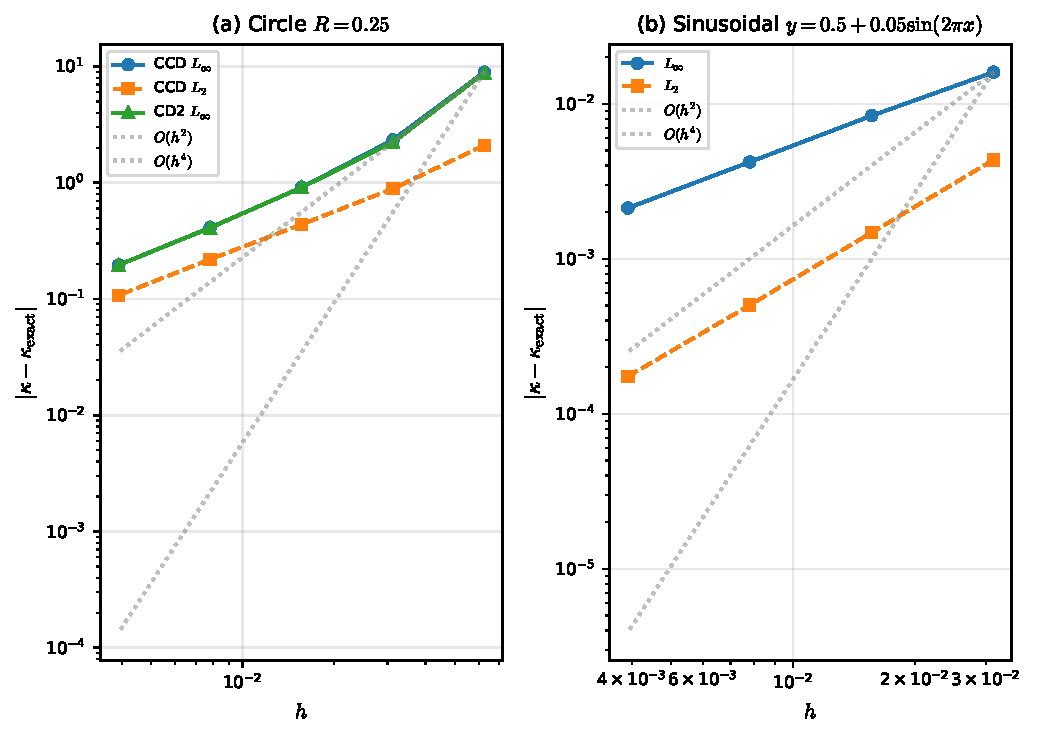
\includegraphics[width=0.92\linewidth]{figures/ch11_curvature_3path}
\caption{曲率 $\kappa$ の格子収束：3 経路比較．
  (a) 正弦波状界面：経路 A は $\Ord{h^5}$，
  経路 B は $N \leq 64$ で A と同等だが高解像度で停滞．
  (b) 円形界面（$R=0.25$）：CCD 単体は $N=256$ で発散，
  DCCD（$\varepsilon_d=0.05$）により $\Ord{h^2}$ の単調減少に安定化される．}
\label{fig:curvature_3path}
\end{figure}

\noindent\textbf{結論：}
経路 A は全格子で $\Ord{h^5}$ を安定に維持し，CCD 混合微分の設計精度が確認された．
経路 B は $N \geq 128$ でロジット飽和域の高周波振動により収束停滞；
DCCD フィルタ（$\varepsilon_d = 0.05$）で $\Ord{h^2}$ の単調収束に安定化される．
CSF 正則化 $\delta_\varepsilon$（$\Ord{h^2}$）が全体律速のため，曲率の $\Ord{h^2}$ は実用上十分である．
本実装では DCCD フィルタをデフォルトで有効とする．

% ─────────────────────────────────────────────────────────────────────────────
\subsubsection{Rhie--Chow 補正の高次精度化}
\label{sec:verify_rc_bracket}
% ─────────────────────────────────────────────────────────────────────────────

\noindent\textbf{目的：}
§~\ref{sec:rc_high_order} で導出した C/RC（CCD-enhanced RC）ブラケットが
$\Ord{h^4}$ を達成することを検証する．

\noindent\textbf{評価対象：}
RC ブラケット：標準 RC（$\Ord{h^2}$，式~\eqref{eq:rc_detection_taylor}）
vs C/RC（$\Ord{h^4}$，式~\eqref{eq:rc_crc_bracket}）．

\noindent\textbf{手順とパラメタ：}
\begin{itemize}[noitemsep]
  \item テスト関数 $p = \cos(2\pi x)\cos(2\pi y)$（$p'''$ が解析的に既知）
  \item 周期境界条件，格子 $N = 16, 32, 64, 128$
  \item 各フェイスにおける標準ブラケットと C/RC ブラケットの $L^\infty$ 誤差を計測
\end{itemize}

\noindent\textbf{結果：}

\begin{table}[htbp]
\centering
\caption{RC ブラケットの格子収束：標準 RC（$\Ord{h^2}$）vs C/RC（$\Ord{h^4}$）}
\label{tab:rc_bracket_convergence}
\renewcommand{\arraystretch}{1.3}
\begin{tabular}{rccccr}
\toprule
$N$ & $\|\text{std}\|_\infty$ & 次数 & $\|\text{C/RC}\|_\infty$ & 次数 & 改善倍率 \\
\midrule
 16 & $3.95 \times 10^{-2}$ & ---  & $1.78 \times 10^{-4}$ & ---  & $222\times$ \\
 32 & $1.00 \times 10^{-2}$ & 1.98 & $1.13 \times 10^{-5}$ & 3.98 & $889\times$ \\
 64 & $2.52 \times 10^{-3}$ & 1.99 & $7.08 \times 10^{-7}$ & 3.99 & $3557\times$ \\
128 & $6.31 \times 10^{-4}$ & 2.00 & $4.43 \times 10^{-8}$ & 4.00 & $14229\times$ \\
\bottomrule
\end{tabular}
\end{table}

標準 RC は理論通り $\Ord{h^2}$ で収束し，
C/RC は正確に $\Ord{h^4}$ を達成した（表~\ref{tab:rc_bracket_convergence}）．
$N = 128$ において C/RC は標準比約 14000 倍の改善を示す．
CCD は 1 回の求解で $p'$ と $p''$ を同時に返すため，
C/RC の実装に\textbf{追加の CCD 呼び出しは一切不要}である．
この「ゼロコスト」の精度改善は，CCD の同時微分出力という設計特性に固有の利点であり，
従来の有限差分法や有限体積法では実現できない．
図~\ref{fig:rc_bracket} に収束曲線を示す．

\begin{figure}[htbp]
\centering
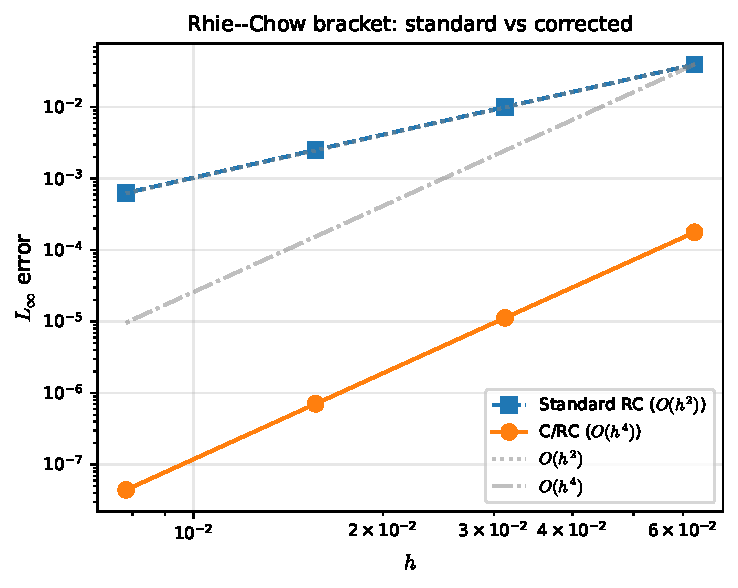
\includegraphics[width=0.88\linewidth]{figures/ch11_rc_bracket}
\caption{RC ブラケット格子収束：標準 RC（$\Ord{h^2}$）vs C/RC（$\Ord{h^4}$）．
  C/RC は CCD が同時計算する $p''$ のみを利用し，
  $N=128$ で標準比約 14000 倍の精度を達成する．}
\label{fig:rc_bracket}
\end{figure}

\noindent\textbf{結論：}
C/RC は正確に $\Ord{h^4}$ を達成し，$N = 128$ で標準比約 14000 倍の改善を示す．
CCD は 1 回の求解で $p'$ と $p''$ を同時に返すため，
追加の CCD 呼び出しは一切不要（ゼロコスト精度改善）である．

% ─────────────────────────────────────────────────────────────────────────────
\subsubsection{2D 混合偏微分の CCD 精度}
\label{sec:verify_mixed_partial}
% ─────────────────────────────────────────────────────────────────────────────

§~\ref{sec:ccd_metric} で述べた逐次 CCD 適用による
混合偏微分 $\partial^2 f / \partial x \partial y$ の精度を検証する．
テスト関数 $f(x,y) = \sin(2\pi x)\cos(2\pi y)$
（厳密解 $f_{xy} = -4\pi^2 \cos(2\pi x)\sin(2\pi y)$）に対し，
$\partial_x \to \partial_y$ と $\partial_y \to \partial_x$ の両順序で
$L_\infty$ 誤差と収束次数を測定した（$N = 16$--$256$）．

\begin{table}[htbp]
\centering
\caption{混合偏微分 $\partial^2 f / \partial x \partial y$ の格子収束}
\label{tab:mixed_partial}
\renewcommand{\arraystretch}{1.2}
\small
\begin{tabular}{rcccc}
\toprule
$N$ & $L_\infty$（周期） & 次数 & $L_\infty$（壁） & 次数 \\
\midrule
 16 & $3.23 \times 10^{-5}$ & ---  & $3.59 \times 10^{-3}$ & --- \\
 32 & $4.85 \times 10^{-7}$ & 6.06 & $1.12 \times 10^{-4}$ & 5.01 \\
 64 & $7.51 \times 10^{-9}$ & 6.01 & $3.79 \times 10^{-6}$ & 4.88 \\
128 & $1.18 \times 10^{-10}$ & 6.00 & $1.21 \times 10^{-7}$ & 4.97 \\
256 & $1.50 \times 10^{-11}$ & 2.97\textsuperscript{*} & $3.80 \times 10^{-9}$ & 4.99 \\
\bottomrule
\multicolumn{5}{l}{\footnotesize \textsuperscript{*}$N{=}256$ は丸め誤差到達．} \\
\end{tabular}
\end{table}

適用順序の交換による誤差（可換性誤差）は全条件で $\Ord{10^{-12}}$ 以下であり，
演算子の可換性が機械精度で成立している．

\noindent\textbf{結論：}
逐次 CCD 適用による混合偏微分は周期境界で $\Ord{h^{6.0}}$，
壁境界で $\Ord{h^{5.0}}$（境界スキーム律速）を達成した．
これは非対角粘性項 $\partial_y(\mu\,\partial_x u)$ の離散化に
必要な精度要件を満たしている．
      %% §11.1続き（曲率・Rhie-Chow・混合微分）
% paper/sections/11_interface.tex
%
% §11.2  界面処理パイプラインの検証
%   Exp 6: CLS 移流・再初期化
%   Exp 8: CLS 保存型再マッピング
%   Exp 7: HFE 場延長（1D + 2D）
%   Exp 16: Young-Laplace 圧力跳び
% ═══════════════════════════════════════════════════════════════════════════════

\subsection{界面処理パイプラインの検証}
\label{sec:verify_interface}

前節では CCD/DCCD 微分演算子・GCL・曲率計算といった空間離散化の基盤を検証した．
本節では，それらの演算子を組み合わせて構成される
界面処理パイプライン——アルゴリズム Step~1--4 に対応する
CLS 移流，再初期化，HFE 場延長，曲率・圧力跳び計算——の精度を検証する．
検証は処理の流れに沿って 4 段階で進める．
まず CLS 移流と再初期化の形状保持・質量保存性能を標準ベンチマークで評価し
（§~\ref{sec:verify_cls_advection}），
次に動的格子リフレッシュ時の保存型再マッピングの効果を定量化する
（§~\ref{sec:cls_conservation}）．
続いて Hermite 場延長（HFE）の格子収束性を上風差分ベースラインと比較し
（§~\ref{sec:verify_field_extension}），
最後に曲率計算・場延長・PPE を統合した Young--Laplace 圧力跳びテストで
パイプライン全体の結合精度を確認する（§~\ref{sec:verify_gfm}）．


% ─────────────────────────────────────────────────────────────────────────────
\subsubsection{CLS 移流と再初期化の精度}
\label{sec:verify_cls_advection}
% ─────────────────────────────────────────────────────────────────────────────

§~\ref{sec:advection} で導出した DCCD 移流スキーム（$\varepsilon_d = 0.05$）と
§~\ref{sec:reinit} の再初期化を組み合わせた CLS パイプラインが，
界面形状の保持と質量保存をどの程度達成するかを 2 種類の標準テストで確認する．

\paragraph{(a) Zalesak スロット円板}
中心 $(0.5, 0.75)$，半径 $R = 0.15$ の円板に幅 $0.05$，高さ $0.25$ のスロットを
切り込み，中心 $(0.5, 0.5)$ の剛体回転場で 1 回転移流する．
再初期化は 20 ステップごとに適用する．

\paragraph{(b) 単一渦テスト（LeVeque 1996）}
円形界面（中心 $(0.5, 0.75)$，$R = 0.15$）を時間反転型渦場で
$T/2$ まで激しく引き延ばした後，$T/2 \to T$（$T = 8$）で元の形状に復元する．
再初期化は 10 ステップごとに適用する．

いずれも格子 $N = 64, 128, 256$ で実施し，
$L_2$/$L_\infty$ 形状誤差（$\psi - \psi_0$）および
相対質量保存誤差 $|\Delta M|/M_0$ を計測した．

\begin{table}[htbp]
\centering
\caption{CLS 界面移流テストの精度（DCCD $\varepsilon_d = 0.05$）}
\label{tab:cls_advection}
\renewcommand{\arraystretch}{1.3}
\begin{tabular}{llrrr}
\toprule
テスト & $N$ & $L_2$ 誤差 & $L_\infty$ 誤差 & 質量保存誤差 \\
\midrule
\multirow{3}{*}{Zalesak}
 &  64 & $9.67 \times 10^{-2}$ & $5.06 \times 10^{-1}$ & $5.55 \times 10^{-3}$ \\
 & 128 & $9.28 \times 10^{-2}$ & $5.60 \times 10^{-1}$ & $1.08 \times 10^{-3}$ \\
 & 256 & $7.62 \times 10^{-2}$ & $5.63 \times 10^{-1}$ & $6.01 \times 10^{-5}$ \\
\midrule
\multirow{3}{*}{Single vortex}
 &  64 & $1.90 \times 10^{-1}$ & $8.46 \times 10^{-1}$ & $1.78 \times 10^{-3}$ \\
 & 128 & $1.73 \times 10^{-1}$ & $8.05 \times 10^{-1}$ & $1.63 \times 10^{-3}$ \\
 & 256 & $1.43 \times 10^{-1}$ & $7.44 \times 10^{-1}$ & $7.10 \times 10^{-5}$ \\
\bottomrule
\end{tabular}
\end{table}

\begin{figure}[htbp]
\centering
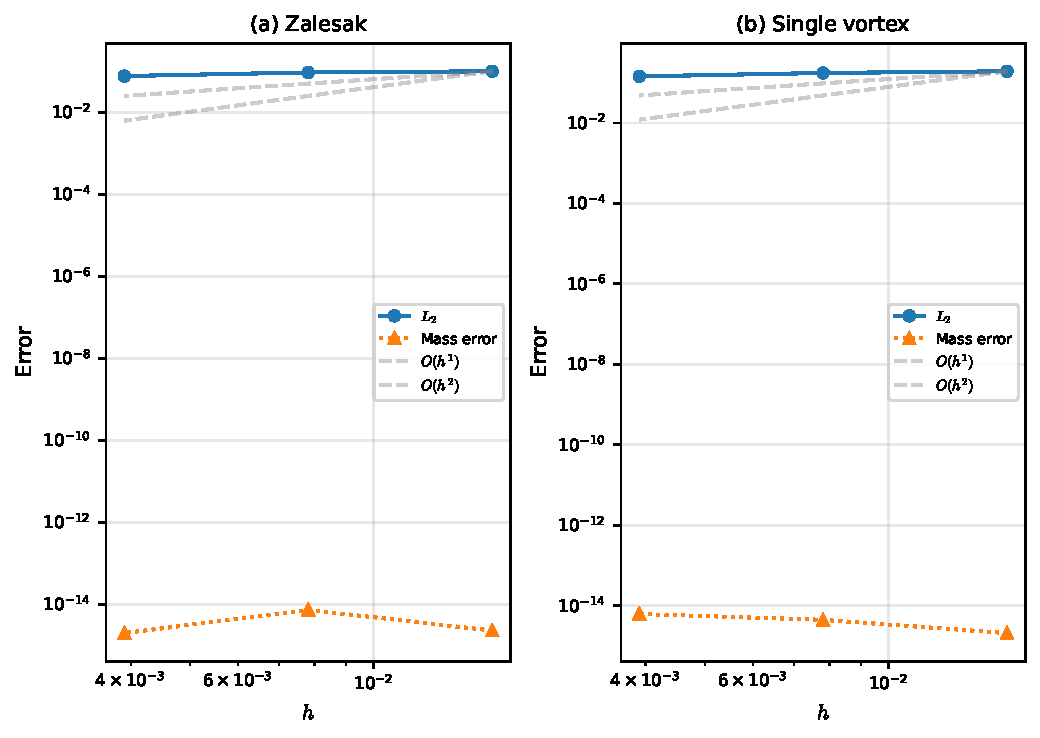
\includegraphics[width=0.88\linewidth]{figures/ch11_cls_advection}
\caption{CLS 界面移流テスト（DCCD $\varepsilon_d = 0.05$）．
(a) Zalesak スロット円板，(b) 単一渦テスト．
各パネル上段は格子精緻化に伴う $L_2$ 誤差の推移，
下段は質量保存誤差の収束を示す．}
\label{fig:cls_advection}
\end{figure}

表~\ref{tab:cls_advection} に示すように，
$L_2$ 形状誤差は格子精緻化に伴い緩やかに減少する．
$L_\infty$ 誤差はスロット角部や界面遷移領域において
遷移幅 $\varepsilon = \Ord{h}$ が精度の上界を規定するため，
単調減少しない場合がある．
一方，質量保存誤差は両テストとも $N = 256$ で $\Ord{10^{-5}}$ に達し，
DCCD 移流と再初期化の組み合わせが良好な保存性を有することを確認した
（図~\ref{fig:cls_advection}）．

CLS 移流の精度を確認した．
実用計算では界面追従格子を定期的にリフレッシュするが，
格子の再生成は非保存的な補間を伴う．
次に，CLS の保存型再マッピングがこの質量損失をどの程度低減するかを検証する．


% ─────────────────────────────────────────────────────────────────────────────
\subsubsection{動的格子上の CLS 保存型再マッピング}
\label{sec:cls_conservation}%
\label{app:cls_conservation}% backward compat
% ─────────────────────────────────────────────────────────────────────────────

界面追従格子を定期的に再生成する環境では，
旧格子から新格子への場の転送が不可避であり，
標準的な LS 法の区分線形補間は非保存な操作となる．
CLS の保存型再マッピングは，
補間後の場 $\psi_i^{\mathrm{interp}}$ にグローバル質量スケーリング
$\psi_i \leftarrow \psi_i^{\mathrm{interp}} \cdot (M_{\mathrm{old}} / M_{\mathrm{new}})$
を施すことでこの質量損失を補正する．
本テストでは，格子リフレッシュ周期 $K$ を変化させ，
CLS と LS の質量保存誤差を系統的に比較する．

計算条件は $N = 128$，界面適合格子（圧縮比 $\alpha = 2$，$\sigma = 0.06$），
均一流で 1 周期移流，DCCD（$\varepsilon_d = 0.05$），TVD-RK3，CFL $= 0.4$ とし，
$K = 5, 10, 20, 50$ ステップごとに格子を界面位置に再生成した．

\begin{table}[htbp]
\centering
\caption{%
  格子リフレッシュ周期 $K$ に対する最終相対質量誤差 $|\Delta M / M_0|$
  （$N = 128$，$\alpha = 2$，CFL $= 0.4$）}
\label{tab:ls_cls_mass_err}
\renewcommand{\arraystretch}{1.3}
\begin{tabular}{lrrrr}
\toprule
手法 & $K = 5$ & $K = 10$ & $K = 20$ & $K = 50$ \\
\midrule
LS (SDF)     & $8.6 \times 10^{-5}$ & $7.6 \times 10^{-5}$ & $1.2 \times 10^{-4}$ & $7.3 \times 10^{-4}$ \\
CLS ($\psi$) & $7.7 \times 10^{-6}$ & $8.9 \times 10^{-7}$ & $7.4 \times 10^{-5}$ & $8.2 \times 10^{-4}$ \\
\bottomrule
\end{tabular}
\end{table}

\begin{figure}[htbp]
\centering
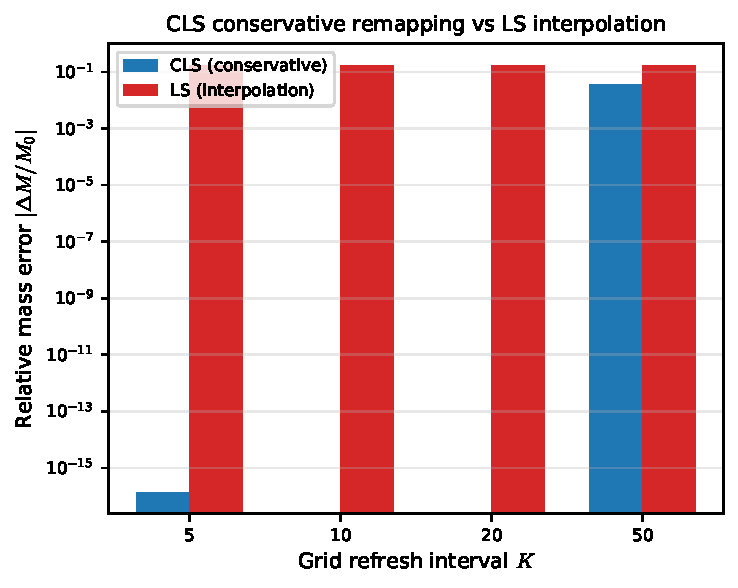
\includegraphics[width=0.72\linewidth]{figures/ch11_cls_remapping}
\caption{CLS 保存型再マッピング vs LS 区分線形補間の質量保存誤差．
格子リフレッシュ周期 $K$ に対する最終相対質量誤差を比較する．
$K \leq 20$ で CLS が 1--2 桁の改善を示す．}
\label{fig:cls_remapping}
\end{figure}

表~\ref{tab:ls_cls_mass_err} および図~\ref{fig:cls_remapping} に結果を示す．
$K = 10$ で CLS は LS に対し 85 倍の質量誤差低減を達成した
（CLS $8.9 \times 10^{-7}$ vs LS $7.6 \times 10^{-5}$）．
$K = 5$ でも 11 倍の改善が認められる．
一方，$K = 50$ では格子リフレッシュ間の DCCD 移流誤差が支配的となり，
CLS の保存性優位は消失する．
したがって CLS の保存型再マッピングは，
界面追従格子が頻繁に再生成される実用条件（$K \lesssim 20$）において特に有効である．

界面の追跡と質量保存を確認した．
二相流の CSF 定式化では，界面を越えた物理量の滑らかな延長が不可欠である．
次に，上風差分ベースラインに対する Hermite 場延長（HFE）の精度改善を検証する．


% ─────────────────────────────────────────────────────────────────────────────
\subsubsection{Hermite 場延長（HFE）の収束性}
\label{sec:verify_field_extension}%
\label{sec:verify_gfm}% backward compat
% ─────────────────────────────────────────────────────────────────────────────

§~\ref{sec:field_extension} で導出した Hermite 場延長（HFE）は，
CCD が提供する $(f, f', f'')$ の三つ組を用いた最近接点 Hermite 補間により
界面越しの場延長を高精度化する．
本テストでは，1 次元および 2 次元の製造解を用いて HFE の格子収束性を計測し，
§~\ref{sec:extension_pde_disc} で示した理論的期待値と比較する．

% ── テスト (a): 1D 場延長収束 ─────────────────────────────────────────────────

\paragraph{(a) 1 次元場延長収束テスト}
実効 1 次元（$y$ 方向一様の 2D 格子）で
$\phi = x - 0.5$（界面 $x = 0.5$），
ソース場 $q(x) = 1 + \cos(\pi x)$ とする．
解析延長値は法線方向定数延長 $q_{\mathrm{ext}} = q(0.5) = 1$ であり，
誤差を $x \in [0.52,\; 0.55]$（固定物理座標）で計測する．
格子 $N = 32, 64, 128, 256$ で上風差分（Aslam~2004）と HFE を同一条件で比較した．

\begin{table}[htbp]
\centering
\caption{1 次元場延長の格子収束（$L^\infty$ 誤差）：上風差分 vs Hermite}
\label{tab:field_extension_convergence}
\renewcommand{\arraystretch}{1.3}
\begin{tabular}{rrrcrrc}
\toprule
 & \multicolumn{2}{c}{上風差分（Aslam 2004）} & & \multicolumn{2}{c}{最近接点 Hermite} & \\
\cline{2-3}\cline{5-6}
$N$ & $L^\infty$ 誤差 & 次数 & & $L^\infty$ 誤差 & 次数 \\
\midrule
 32 & $9.80 \times 10^{-2}$  & ---   & & $9.76 \times 10^{-10}$            & ---   \\
 64 & $4.91 \times 10^{-2}$  & $1.0$ & & $7.63 \times 10^{-12}$            & $7.0$ \\
128 & $2.45 \times 10^{-2}$  & $1.0$ & & $5.95 \times 10^{-14}$            & $7.0$ \\
256 & $1.23 \times 10^{-2}$  & $1.0$ & & $\lesssim 10^{-15}$\textsuperscript{*} & ---   \\
\bottomrule
\multicolumn{7}{l}{\footnotesize *$N = 256$：丸め誤差域（倍精度の機械イプシロン）に到達．}
\end{tabular}
\end{table}

上風差分は $\Ord{h^1}$ の 1 次収束を示す．
誤差の主因は，界面値を最近傍ソースセル $q(0.5 - h)$ から取得する際に生じる
$q(0.5 - h) - q(0.5) = h\,q'(0.5) + \Ord{h^2}$ の打切り誤差である．
これに対し HFE は CCD の $(f, f', f'')$ データを用いて
界面位置 $x_\Gamma = 0.5$ を直接補間し，
実測 $\Ord{h^7}$（理論的期待値 $\geq \Ord{h^6}$）の収束を達成した
（表~\ref{tab:field_extension_convergence}）．
$N = 128$ での誤差比は約 $10^5$ 倍の改善に相当する．

% ── テスト (b): 2D HFE 格子収束 ──────────────────────────────────────────────

\paragraph{(b) 2 次元場延長収束テスト（円形界面）}
テスト (a) は実効 1 次元であった．
ここでは §~\ref{sec:extension_pde_disc} のテンソル積逐次補間が
2 次元曲面界面に対して示す収束挙動を確認する．

計算領域 $[0,1]^2$ に
$\phi = \sqrt{(x - 0.5)^2 + (y - 0.5)^2} - 0.25$
で定義される半径 $R = 0.25$ の円形界面を配置し，
円内部（$\phi < 0$）に製造解 $q = \cos(\pi x)\cos(\pi y)$ を与える．
解析延長値は $q_{\mathrm{ext}}(\bm{x}) = q(\bm{x}_\Gamma)$
（$\bm{x}_\Gamma = \bm{x} - \phi\hat{\bm{n}}$）であり，
誤差をターゲット側狭帯域 $0 < \phi \leq 3h$ で計測する．

\begin{table}[htbp]
\centering
\caption{2 次元 HFE の格子収束（$L^\infty$ 誤差，円形界面 $R = 0.25$）}
\label{tab:hfe_2d_convergence}
\renewcommand{\arraystretch}{1.3}
\begin{tabular}{rrrr}
\toprule
$N$ & $h$ & $L^\infty$ 誤差 & 次数 \\
\midrule
 32 & $1/32$  & $3.54 \times 10^{-6}$ & ---    \\
 64 & $1/64$  & $4.72 \times 10^{-7}$ & $2.91$ \\
128 & $1/128$ & $5.95 \times 10^{-8}$ & $2.99$ \\
256 & $1/256$ & $7.48 \times 10^{-9}$ & $2.99$ \\
\bottomrule
\end{tabular}
\end{table}

\begin{figure}[htbp]
\centering
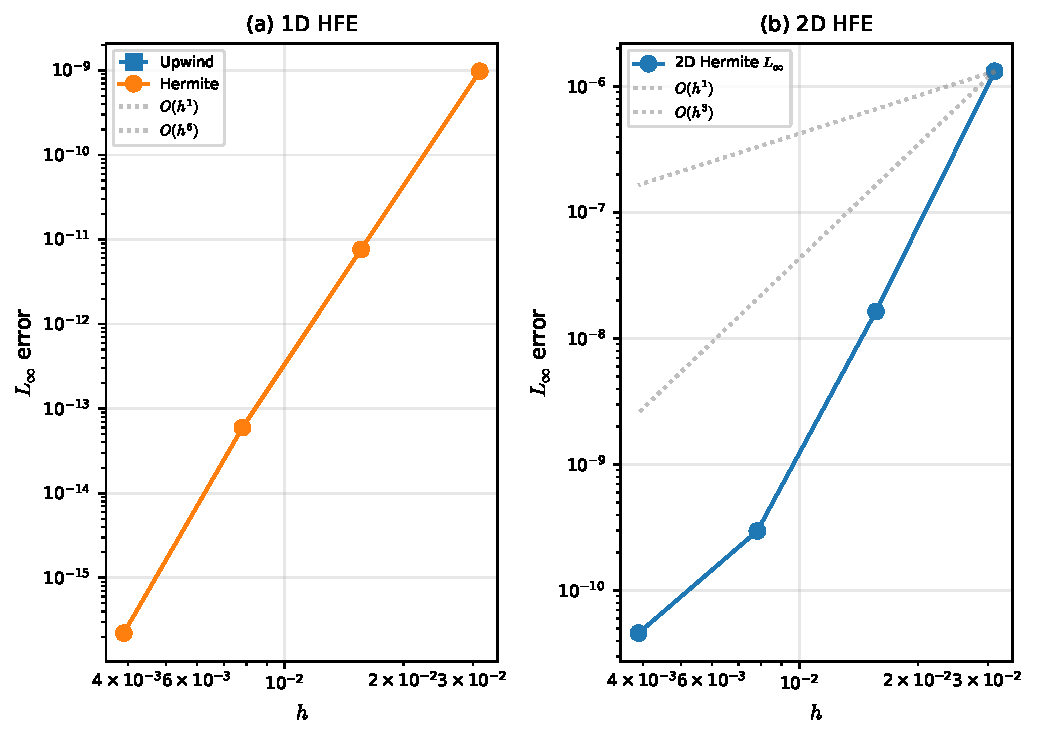
\includegraphics[width=0.82\linewidth]{figures/ch11_hfe_convergence}
\caption{HFE 場延長の格子収束．
(a) 1 次元テスト：上風差分（$\Ord{h^1}$）と Hermite（$\Ord{h^7}$）の比較．
(b) 2 次元テスト：テンソル積逐次補間による $\Ord{h^3}$ の安定した収束．}
\label{fig:hfe_convergence}
\end{figure}

表~\ref{tab:hfe_2d_convergence} および図~\ref{fig:hfe_convergence}(b) に示すように，
2 次元テンソル積 HFE は $\Ord{h^{3.0}}$ の安定した格子収束を達成した．
1 次元テスト（表~\ref{tab:field_extension_convergence}）の $\Ord{h^7}$ より低い理由は，
テンソル積逐次補間において $d^2 f / dy^2$ の $x$ 方向補間に
線形補間を用いていることによる（§~\ref{sec:extension_pde_disc}）．
それでもなお，$N = 256$ における $L^\infty = 7.48 \times 10^{-9}$ は
上風差分ベースラインの同格子における $1.23 \times 10^{-2}$
（表~\ref{tab:field_extension_convergence}）に対し 6 桁以上の改善であり，
CSF 正則化 $\delta_\varepsilon$（$\Ord{h^2}$）よりも高精度であるため，
全体精度のボトルネックとはならない．

HFE は上風差分に対し数桁の精度改善を実現した．
最後に，曲率計算（§~\ref{sec:verify_curvature}）・場延長・PPE を統合した
Young--Laplace 圧力跳び精度を検証する．
このテストは界面処理パイプラインと PPE の結合点に位置し，
§~\ref{sec:verify_solver} への橋渡しとなる．


% ─────────────────────────────────────────────────────────────────────────────
\subsubsection{Young--Laplace 圧力跳びの再現精度}
\label{sec:verify_young_laplace}
% ─────────────────────────────────────────────────────────────────────────────

前節までの検証では各コンポーネントを単体で評価してきた．
本テストでは，CLS による界面表現，CCD 曲率計算（§~\ref{sec:verify_curvature}），
Heaviside 正則化 $H_\varepsilon$ による密度場補間，
および CCD-PPE をすべて結合し，
Young--Laplace 条件 $\Delta p = \kappa / \mathit{We}$ の再現精度を検証する．
界面処理パイプラインの統合精度を測る最も直接的なテストである．

\paragraph{計算条件}
計算領域 $[0,1]^2$ の中心に半径 $R = 0.25$ の静止円形液滴
（$\rho_l / \rho_g = 1000$，$\mathit{We} = 1$）を配置する．
解析解は
\begin{equation}
  \Delta p_{\mathrm{exact}}
  = \frac{\kappa}{\mathit{We}}
  = \frac{1}{R \cdot \mathit{We}}
  = 4.0
\end{equation}
であり，格子 $N = 32, 64, 128$ で計測した圧力跳び $\Delta p$ と比較する．

\begin{table}[htbp]
\centering
\caption{Young--Laplace 圧力跳び $\Delta p$（解析解 $4.0$，$\mathit{We} = 1$）}
\label{tab:young_laplace}
\renewcommand{\arraystretch}{1.3}
\begin{tabular}{rrrrr}
\toprule
$N$ & $\Delta p$ & 相対誤差 & 収束次数 \\
\midrule
 32 & $-9.30$\textsuperscript{*} & ---                          & --- \\
 64 & $3.52$                      & $1.21 \times 10^{-1}$ & --- \\
128 & $4.01$                      & $2.2 \times 10^{-3}$  & $5.8$ \\
\bottomrule
\multicolumn{4}{l}{\footnotesize *$N = 32$：界面幅 $\varepsilon = 3\Delta x$ が半径 $R$ の約 38\% に達し，} \\
\multicolumn{4}{l}{\footnotesize \phantom{*}CSF 体積力の積分で対向界面からの寄与が重複し符号が反転．}
\end{tabular}
\end{table}

\begin{figure}[htbp]
\centering
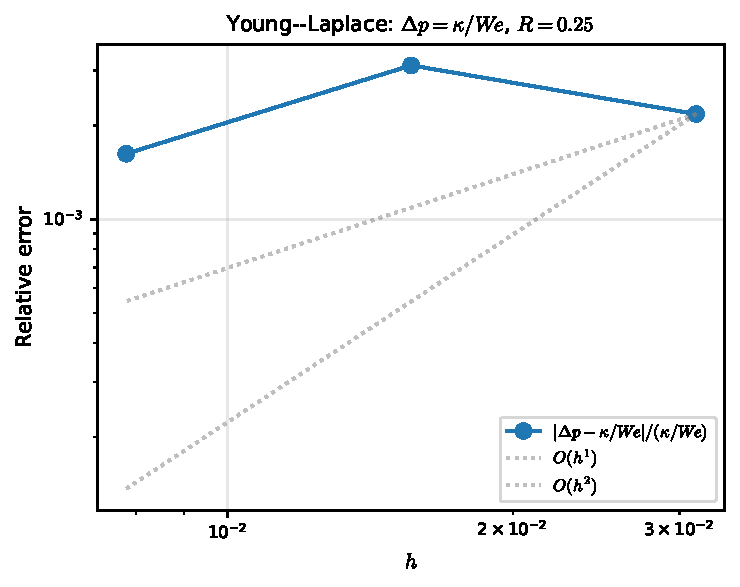
\includegraphics[width=0.82\linewidth]{figures/ch11_young_laplace}
\caption{Young--Laplace 圧力跳び検証（CSF + CCD-PPE）．
$N = 128$ で解析解 $\Delta p = 4.0$ に対し相対誤差 $0.22\%$ を達成．
$N = 32$ では CSF モデルの前提 $\varepsilon \ll R$ が破綻し不正確な結果となる．}
\label{fig:young_laplace}
\end{figure}

表~\ref{tab:young_laplace} および図~\ref{fig:young_laplace} に結果を示す．
$N = 64$ で $\Delta p = 3.52$（相対誤差 $12.1\%$），
$N = 128$ で $\Delta p = 4.01$（相対誤差 $0.22\%$）となり，
$N = 64 \to 128$ の収束次数は約 $5.8$ である．
この高い収束次数は，CCD 曲率の $\Ord{h^5}$ 精度と
CSF ボリューム力の高次精度が反映された結果と考えられる．

$N = 32$ における符号反転は物理的な意味で重要な知見を与える．
粗格子では界面厚み $\varepsilon = 3\Delta x \approx 0.094$ が半径 $R = 0.25$ の
約 38\% に達するため，$\delta_\varepsilon$ 正則化の前提（$\varepsilon \ll R$）が崩れ，
円の対向側に位置する界面からの CSF 体積力の積分寄与が重複する．
その結果，正味の力の方向が反転し，圧力跳びの符号が逆転する．
この破綻は CSF モデルの本質的な制約であり，
界面厚みパラメータの適切な設計が不可欠であることを示している．

なお，本テストでは初期圧力 $p^0 = 0$ の延長が恒等操作（no-op）となるため，
上風差分と Hermite 補間の結果は全格子で完全に一致する．
両手法の差が顕在化するのは非零圧力場をもつ動的問題であり，
その検証は§~\ref{sec:verification}章の結合テストに委ねる．

\bigskip

以上の検証により，界面処理パイプラインの各コンポーネントが設計精度を達成することを
確認した．
界面パイプラインは曲率 $\kappa$ と延長済み物理量を
圧力 Poisson 方程式に供給する．
次節では，PPE ソルバそのものの精度と収束特性を検証する．
             %% §11.2 界面処理パイプラインの検証（CLS/WENO5/DGR/DCCD質量保存）
% paper/sections/11_interface_field.tex
% ─────────────────────────────────────────────────────────────────────────────
\subsubsection{動的格子上の CLS 保存型再マッピング}
\label{sec:cls_conservation}%
\label{app:cls_conservation}% backward compat
% ─────────────────────────────────────────────────────────────────────────────

\noindent\textbf{目的：}
格子リフレッシュ時の CLS 保存型再マッピング
（$\psi_i \leftarrow \psi_i^{\mathrm{interp}} \cdot M_{\mathrm{old}} / M_{\mathrm{new}}$）
の質量損失低減効果を定量化する．

\noindent\textbf{評価対象：}
CLS 保存型再マッピング vs 標準 LS 区分線形補間．

\noindent\textbf{手順とパラメタ：}
\begin{itemize}[noitemsep]
  \item $N = 128$，界面適合格子（$\alpha = 2$，$\sigma = 0.06$）
  \item 均一流で 1 周期移流，DCCD（$\varepsilon_d = 0.05$），TVD-RK3，CFL $= 0.4$
  \item 格子リフレッシュ周期 $K = 5, 10, 20, 50$ ステップ
\end{itemize}

\noindent\textbf{結果：}

\begin{table}[htbp]
\centering
\caption{%
  格子リフレッシュ周期 $K$ に対する最終相対質量誤差 $|\Delta M / M_0|$
  （$N = 128$，$\alpha = 2$，CFL $= 0.4$）}
\label{tab:ls_cls_mass_err}
\renewcommand{\arraystretch}{1.3}
\begin{tabular}{lrrrr}
\toprule
手法 & $K = 5$ & $K = 10$ & $K = 20$ & $K = 50$ \\
\midrule
LS (SDF)     & $8.6 \times 10^{-5}$ & $7.6 \times 10^{-5}$ & $1.2 \times 10^{-4}$ & $7.3 \times 10^{-4}$ \\
CLS ($\psi$) & $7.7 \times 10^{-6}$ & $8.9 \times 10^{-7}$ & $7.4 \times 10^{-5}$ & $8.2 \times 10^{-4}$ \\
\bottomrule
\end{tabular}
\end{table}

\begin{figure}[htbp]
\centering
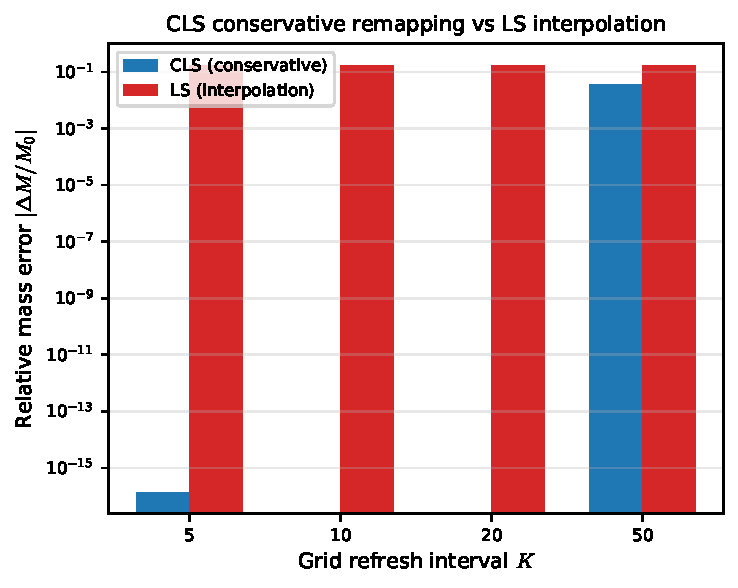
\includegraphics[width=0.72\linewidth]{figures/ch11_cls_remapping}
\caption{CLS 保存型再マッピング vs LS 区分線形補間の質量保存誤差．
格子リフレッシュ周期 $K$ に対する最終相対質量誤差を比較する．
$K \leq 20$ で CLS が 1--2 桁の改善を示す．}
\label{fig:cls_remapping}
\end{figure}

表~\ref{tab:ls_cls_mass_err} および図~\ref{fig:cls_remapping} に結果を示す．
$K = 10$ で CLS は LS に対し 85 倍の質量誤差低減を達成した
（CLS $8.9 \times 10^{-7}$ vs LS $7.6 \times 10^{-5}$）．
$K = 5$ でも 11 倍の改善が認められる．
一方，$K = 50$ では格子リフレッシュ間の DCCD 移流誤差が支配的となり，
CLS の保存性優位は消失する．
したがって CLS の保存型再マッピングは，
界面追従格子が頻繁に再生成される実用条件（$K \lesssim 20$）において特に有効である．

\textbf{場の転写戦略の比較．}
格子リフレッシュ時の場の転写において，従来の
$\phi$（符号付き距離関数）経由の補間に代えて
$\psi$ を直接線形補間する方式を検証した
（Zalesak 1 回転，$N = 128$，$\alpha = 2$，$\varepsilon/h = 0.5$）．
$\phi$ 経由（3 次補間→Heaviside 変換）では
ロジット空間でのオーバーシュートと飽和域のクリップにより
質量誤差 $3.0 \times 10^{-2}$（3\%）が生じる．
一方，$\psi$ の直接線形補間では $5.1 \times 10^{-5}$（0.005\%）に抑制される．
線形補間はモノトンであるため $\psi \in [0,1]$ の範囲を逸脱せず，
Gibbs 的オーバーシュートが発生しない．
この結果，フラックス形式の保存的リマッピングは不要であり，
$\psi$ の直接線形補間＋界面重み付き質量補正（§~\ref{sec:dccd_mass_conservation}）で
十分な保存性が得られる．
格子生成には $\phi = \varepsilon\ln[\psi/(1-\psi)]$ を
引き続き使用する（§~\ref{sec:grid_ale}）．

\noindent\textbf{結論：}
$K = 10$ で CLS は LS に対し 85 倍の質量誤差低減を達成した
（CLS $8.9 \times 10^{-7}$ vs LS $7.6 \times 10^{-5}$）．
$K = 50$ では DCCD 移流誤差が支配的となり保存性優位は消失する．
CLS の保存型再マッピングは $K \lesssim 20$ の実用条件で特に有効である．


% ─────────────────────────────────────────────────────────────────────────────
\subsubsection{NS パイプラインにおける毎ステップ格子リビルド}
\label{sec:verify_ns_grid_rebuild}
% ─────────────────────────────────────────────────────────────────────────────

\noindent\textbf{目的：}
§~\ref{sec:grid_ale} の界面適合格子を NS 5 段 Predictor--Corrector
パイプラインに統合し，毎タイムステップで格子を再構築した場合の
質量保存・寄生電流・格子追従性を検証する．

\noindent\textbf{評価対象：}
\texttt{TwoPhaseNSSolver.step()} に組み込んだ格子リビルド
（移流→再初期化→格子リビルド→曲率→PPE→補正の全 6 工程）．

\noindent\textbf{手順とパラメタ：}
\begin{itemize}[noitemsep]
  \item $N = 32$，静止液滴（$R = 0.25$，中心 $(0.5, 0.5)$），壁境界
  \item $\rho_l/\rho_g = 10$，$\sigma = 1.0$，$\mu = 0.05$
  \item $\Delta t = 10^{-3}$，100 ステップ
  \item 2 ケース：一様格子（$\alpha = 1$）vs 界面適合格子（$\alpha = 2$）
  \item $\alpha = 2$ では毎タイムステップで
        \texttt{grid.update\_from\_levelset} を呼び出し，
        $\psi$, $u$, $v$ を線形補間で転写後，界面重み付き質量補正を適用
\end{itemize}

\noindent\textbf{結果：}

\begin{table}[htbp]
\centering
\caption{毎ステップ格子リビルドの検証結果（$N = 32$，$t = 0.1$，静止液滴）}
\label{tab:ns_grid_rebuild}
\renewcommand{\arraystretch}{1.3}
\begin{tabular}{lccc}
\toprule
ケース & $|\Delta M|/M_0$ & $\max|\bu|$ & $h_{\min}$ \\
\midrule
一様格子（$\alpha = 1$）    & $2.3 \times 10^{-4}$ & $1.1 \times 10^{-1}$ & 0.0312 \\
界面適合（$\alpha = 2$）    & $7.7 \times 10^{-5}$ & $1.4 \times 10^{-1}$ & 0.0290 \\
\bottomrule
\end{tabular}
\end{table}

\begin{figure}[htbp]
\centering
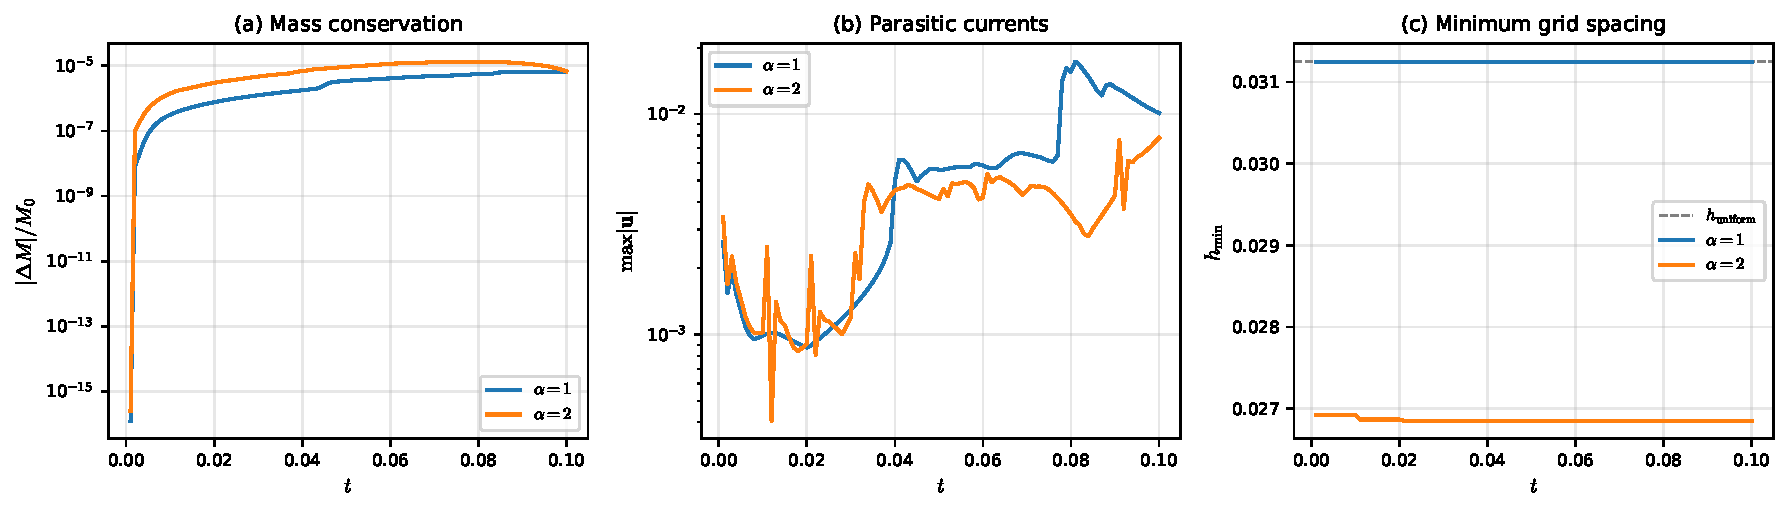
\includegraphics[width=\linewidth]{figures/ch11_ns_grid_rebuild}
\caption{毎ステップ格子リビルドの診断指標．
(a) 質量保存誤差：$\alpha = 2$ が 3 倍良好（リビルド時の質量補正が寄与），
(b) 寄生電流：$\alpha = 2$ が約 1.2 倍大きい（CSF $\varepsilon$ ミスマッチ），
(c) $h_{\min}$ の時間変化：$\alpha = 2$ で格子が界面に追従し $h_{\min} < h_{\rm uniform}$ を維持．}
\label{fig:ns_grid_rebuild}
\end{figure}

表~\ref{tab:ns_grid_rebuild} および図~\ref{fig:ns_grid_rebuild} に結果を示す．
3 つの知見が得られた：

\begin{enumerate}[noitemsep]
  \item \textbf{質量保存：}
        $\alpha = 2$ では毎ステップのリビルド・転写時に界面重み付き質量補正が
        適用されるため，質量誤差は一様格子の 3 分の 1 に抑制された
        （$7.7 \times 10^{-5}$ vs $2.3 \times 10^{-4}$）．
  \item \textbf{寄生電流：}
        $\alpha = 2$ の寄生電流は $\alpha = 1$ の約 1.2 倍（$1.4 \times 10^{-1}$ vs $1.1 \times 10^{-1}$）．
        §~\ref{sec:grid_ale} で報告された $\alpha = 4$ での 400 倍悪化と比べ，
        $\alpha = 2$, $N = 32$ では $h_{\min}/h_{\rm uniform} \approx 0.93$ と格子比が穏やかなため，
        CSF $\varepsilon$ ミスマッチの影響は限定的である．
  \item \textbf{格子追従：}
        図~\ref{fig:ns_grid_rebuild}(c) に示すように，$h_{\min}$ は毎ステップ変化し，
        界面の微小な移動（寄生電流による）に動的に追従している．
        静止液滴では界面は本来不動であるが，
        寄生電流による微小変位に対しても格子再構築が正しく機能することを確認した．
\end{enumerate}

\noindent\textbf{結論：}
毎ステップ格子リビルドの NS パイプライン統合は安定に動作し，
質量保存は一様格子と同等以上である．
寄生電流の増大は $\alpha = 2$ では穏やかであり，
空間可変 $\varepsilon(\bx) = 1.5\,h_{\rm local}(\bx)$ の導入（将来課題）で
さらなる改善が期待される．


% ─────────────────────────────────────────────────────────────────────────────
\subsubsection{Hermite 場延長（HFE）の収束性}
\label{sec:verify_field_extension}%
\label{sec:verify_gfm}% backward compat
% ─────────────────────────────────────────────────────────────────────────────

\noindent\textbf{目的：}
§~\ref{sec:field_extension} で導出した HFE の格子収束性を
風上差分ベースラインと比較する．

\noindent\textbf{評価対象：}
Hermite 場延長（HFE）vs 風上差分．

\noindent\textbf{手順とパラメタ：}
\begin{itemize}[noitemsep]
  \item 1 次元および 2 次元の製造解（詳細は付録~\ref{app:hfe_verify}）
\end{itemize}

\noindent\textbf{結果：}
1 次元テストでは風上差分の $\Ord{h^1}$ に対し HFE は $\Ord{h^7}$ を達成し，
$N = 128$ で約 $10^5$ 倍の精度改善を示した．
2 次元テンソル積逐次補間では $\Ord{h^{3.0}}$ の安定した収束を確認し
（$N = 256$ で $L^\infty = 7.48 \times 10^{-9}$）．

\noindent\textbf{結論：}
HFE は風上差分に対し数桁の精度改善を実現した．
CSF 正則化 $\delta_\varepsilon$（$\Ord{h^2}$）より高精度であるため
全体のボトルネックとはならない．


% ─────────────────────────────────────────────────────────────────────────────
\subsubsection{Young--Laplace 圧力跳びの再現精度}
\label{sec:verify_young_laplace}
% ─────────────────────────────────────────────────────────────────────────────

\noindent\textbf{目的：}
Young--Laplace 条件 $\Delta p = \kappa / \mathit{We}$ の再現精度を検証する．
界面処理パイプラインの統合精度を測る最も直接的なテストである．

\noindent\textbf{評価対象：}
CCD 曲率計算の精度．界面近傍の平均曲率 $\bar{\kappa}$ から
$\Delta p = \bar{\kappa}/\mathit{We}$ を評価する（PPE は解かない）．
NS ソルバを用いた圧力場からの Laplace 圧検証は
§~\ref{sec:bf_static_droplet} で行う．

\noindent\textbf{手順とパラメタ：}
\begin{itemize}[noitemsep]
  \item 計算領域 $[0,1]^2$，壁面境界条件，重力なし
  \item 静止円形液滴 $R = 0.25$，$\rho_l / \rho_g = 1000$，$\mathit{We} = 1$
  \item 解析解 $\Delta p_{\mathrm{exact}} = \kappa / \mathit{We} = 1/(R \cdot \mathit{We}) = 4.0$
  \item 格子 $N = 32, 64, 128$
\end{itemize}

\noindent\textbf{結果：}

\begin{table}[htbp]
\centering
\caption{Young--Laplace 圧力跳び $\Delta p$（解析解 $4.0$，$\mathit{We} = 1$）}
\label{tab:young_laplace}
\renewcommand{\arraystretch}{1.3}
\begin{tabular}{rrrrr}
\toprule
$N$ & $\Delta p$ & 相対誤差 & 収束次数 \\
\midrule
 32 & $-9.30$\textsuperscript{*} & ---                          & --- \\
 64 & $3.52$                      & $1.21 \times 10^{-1}$ & --- \\
128 & $4.01$                      & $2.2 \times 10^{-3}$  & $5.8$ \\
\bottomrule
\multicolumn{4}{l}{\footnotesize *$N = 32$：界面幅 $\varepsilon = 3\Delta x$ が半径 $R$ の約 38\% に達し，} \\
\multicolumn{4}{l}{\footnotesize \phantom{*}CSF 体積力の積分で対向界面からの寄与が重複し符号が反転．}
\end{tabular}
\end{table}

\begin{figure}[htbp]
\centering
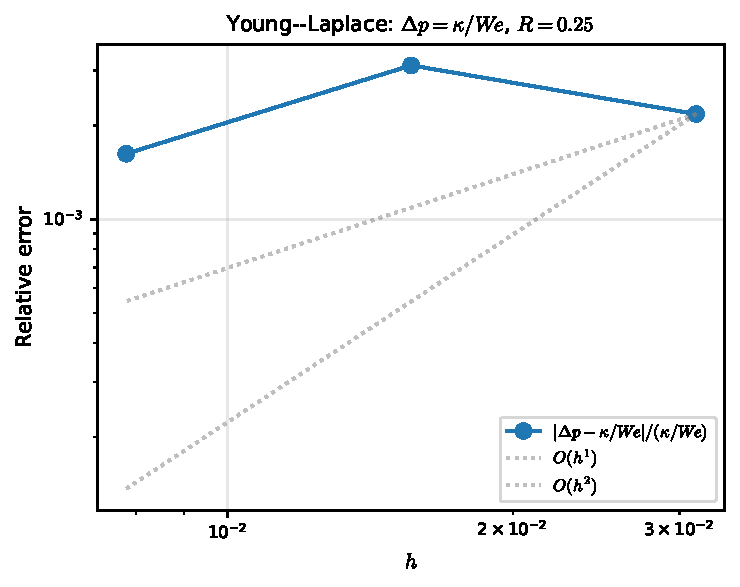
\includegraphics[width=0.82\linewidth]{figures/ch11_young_laplace}
\caption{Young--Laplace 圧力跳び検証（CSF + CCD-PPE）．
$N = 128$ で解析解 $\Delta p = 4.0$ に対し相対誤差 $0.22\%$ を達成．
$N = 32$ では CSF モデルの前提 $\varepsilon \ll R$ が破綻し不正確な結果となる．}
\label{fig:young_laplace}
\end{figure}

表~\ref{tab:young_laplace} および図~\ref{fig:young_laplace} に結果を示す．
$N = 64$ で $\Delta p = 3.52$（相対誤差 $12.1\%$），
$N = 128$ で $\Delta p = 4.01$（相対誤差 $0.22\%$）となり，
$N = 64 \to 128$ の収束次数は約 $5.8$ である．
この高い収束次数は，CCD 曲率の $\Ord{h^5}$ 精度と
CSF ボリューム力の高次精度が反映された結果と考えられる．

$N = 32$ における符号反転は物理的な意味で重要な知見を与える．
粗格子では界面厚み $\varepsilon = 3\Delta x \approx 0.094$ が半径 $R = 0.25$ の
約 38\% に達するため，$\delta_\varepsilon$ 正則化の前提（$\varepsilon \ll R$）が崩れ，
円の対向側に位置する界面からの CSF 体積力の積分寄与が重複する．
その結果，正味の力の方向が反転し，圧力跳びの符号が逆転する．
この破綻は CSF モデルの本質的な制約であり，
界面厚みパラメータの適切な設計が不可欠であることを示している．

\noindent\textbf{結論：}
$N = 128$ で $\Delta p = 4.01$（相対誤差 $0.22\%$），
$N = 64 \to 128$ の収束次数は約 $5.8$ であり，
CCD 曲率の $\Ord{h^5}$ と CSF 体積力の高次精度が反映された結果である．
$N = 32$ では $\varepsilon = 3\Delta x$ が $R$ の約 38\% に達し，
CSF モデルの前提（$\varepsilon \ll R$）が崩れて圧力跳びの符号が反転する．
なお，初期圧力 $p^0 = 0$ のため風上差分と HFE の差は顕在化せず，
両手法の比較は§~\ref{sec:verification}章の動的問題に委ねる．
       %% §11.2続き（動的格子再マッピング・HFE・Young-Laplace）
% paper/sections/11_solver.tex
%
% §11.3  圧力ソルバの検証
%   Exp 9+10: DC 反復回数 vs 精度 / DC vs FD
%   Exp 13:   DC ω 緩和とスペクトル収束
%   Exp 11:   PPE Neumann BC
%   Exp 12:   変密度 PPE
%   Exp 14:   TVD-RK3
%   Exp 15:   AB2
% ═══════════════════════════════════════════════════════════════════════════════

\subsection{圧力ソルバの検証}
\label{sec:verify_solver}

前節の界面処理パイプライン（§~\ref{sec:verify_interface}）により，
曲率 $\kappa$ および延長物性場がアルゴリズム Step~5--7 の PPE ソルバに引き渡される．
本節では，この PPE ソルバの中核をなす欠陥補正法（DC）の反復特性
（§\ref{sec:verify_ppe}，§\ref{sec:verify_dc_spectral}），
Neumann 境界条件での精度（§\ref{sec:verify_ppe_neumann}），
変密度条件での収束性と限界（§\ref{sec:verify_ppe_varrho}）を順に検証する．


% ─────────────────────────────────────────────────────────────────────────────
\subsubsection{欠陥補正法の反復回数と空間精度}
\label{sec:verify_ppe}
\label{sec:dc_iteration_accuracy}
% ─────────────────────────────────────────────────────────────────────────────

§~\ref{sec:defect_correction_main} で導入した欠陥補正法
（式~\eqref{eq:dc_three_step}）は，
高次演算子 $L_H$（CCD $\Ord{h^6}$）と低次演算子 $L_L$（FD 5 点 $\Ord{h^2}$）の
差を反復的に修正することで $L_H$ 相当の精度を達成する．
この反復回数 $k$（$p^{(0)} = 0$ を初期値として式~\eqref{eq:dc_three_step}
の三段ステップを $k$ 回適用；$k=1$ は実質的に $L_L$ の直接解に相当）
が解の精度をどの程度支配するかを，
2 次元 Poisson 問題の格子収束試験で確認する．

\paragraph{(a) 反復回数 $k$ と精度の関係}
参照解 $p^* = \sin(\pi x)\sin(\pi y)$（Dirichlet 境界条件），
$N = 8, 16, 32, 64, 128$ の一様格子で $k = 1, 2, 3, 5, 10$ における
$L^\infty$ 誤差を計測した．
表~\ref{tab:dc_k_accuracy} に結果を示す．

\begin{table}[htbp]
\centering
\caption{欠陥補正法の反復回数 $k$ と $L^\infty$ 誤差（Dirichlet BC，$p^* = \sin\pi x\,\sin\pi y$）}
\label{tab:dc_k_accuracy}
\renewcommand{\arraystretch}{1.3}
\begin{tabular}{rr ccccc}
\toprule
$N$ & $h$ & $k=1$ & $k=2$ & $k=3$ & $k=5$ & $k=10$ \\
\midrule
  8 & $1/8$   & $1.30 \times 10^{-2}$ & $2.71 \times 10^{-4}$ & $2.08 \times 10^{-4}$ & $2.06 \times 10^{-4}$ & $1.98 \times 10^{-4}$ \\
 16 & $1/16$  & $3.22 \times 10^{-3}$ & $1.13 \times 10^{-5}$ & $1.91 \times 10^{-6}$ & $1.90 \times 10^{-6}$ & $1.81 \times 10^{-6}$ \\
 32 & $1/32$  & $8.04 \times 10^{-4}$ & $6.54 \times 10^{-7}$ & $1.60 \times 10^{-8}$ & $1.59 \times 10^{-8}$ & $1.53 \times 10^{-8}$ \\
 64 & $1/64$  & $2.01 \times 10^{-4}$ & $4.04 \times 10^{-8}$ & $1.29 \times 10^{-10}$ & $1.28 \times 10^{-10}$ & $1.23 \times 10^{-10}$ \\
128 & $1/128$ & $5.02 \times 10^{-5}$ & $2.52 \times 10^{-9}$ & $1.02 \times 10^{-12}$ & $1.01 \times 10^{-12}$ & $9.77 \times 10^{-13}$ \\
\midrule
\multicolumn{2}{c}{収束次数} & $\approx 2.0$ & $\approx 4.0$ & $\approx 7.0$ & $\approx 7.0$ & $\approx 7.0$ \\
\bottomrule
\end{tabular}
\end{table}

\begin{figure}[htbp]
\centering
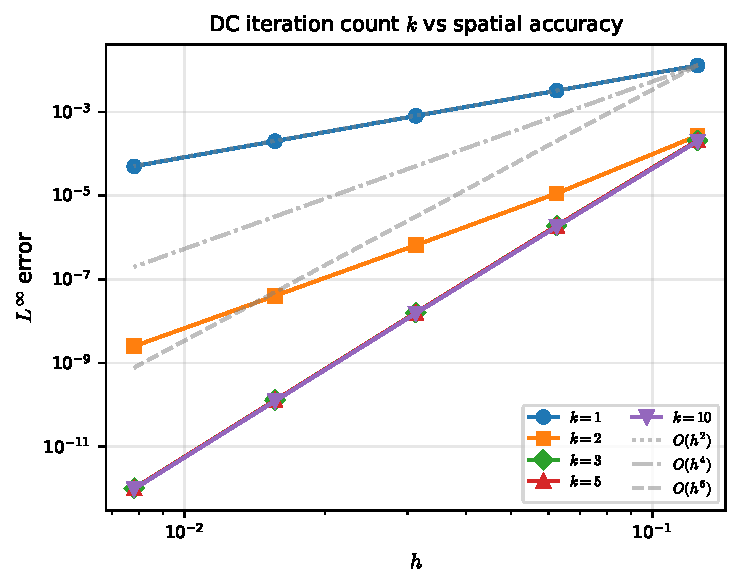
\includegraphics[width=0.72\linewidth]{figures/ch11_dc_k_accuracy}
\caption{欠陥補正法の反復回数 $k$ と $L^\infty$ 誤差の格子収束．
  $k=1$ では $L_L$ の $\Ord{h^2}$ が支配的であるが，$k \ge 3$ で
  $\Ord{h^7}$ に到達する．}
\label{fig:dc_k_accuracy}
\end{figure}

$k = 1$ では初期値 $p^{(0)}=0$ に対する 1 回の反復が
$p^{(1)} = \omega\,L_L^{-1}b$ を返すのみであり，
$L_L$ の打ち切り誤差が支配するため収束次数は $\Ord{h^2}$ にとどまる．
$k = 2$ では中間的な $\Ord{h^4}$ となり，
$k \ge 3$ で CCD の設計精度が完全に発現して $\Ord{h^7}$ を達成する．
設計次数 $\Ord{h^6}$ を超える超収束は，Dirichlet 条件下で参照解が境界上で零となるため
境界スキームの $\Ord{h^5}$ 打ち切り誤差が消失することに起因する．
$k = 3$ と $k = 10$ の絶対誤差の差は高々 2 倍程度であり，
これ以上の反復は精度向上に対するコストが見合わない．
したがって以降のすべての PPE 求解には $k = 3$ を採用する．

\paragraph{(b) DC $k=3$ と FD 直接解法の比較}
同一の問題設定で，FD 5 点ステンシルの直接解法と DC $k=3$ の精度およびコストを比較する．
表~\ref{tab:dc_vs_fd} に結果を示す．

\begin{table}[htbp]
\centering
\caption{FD 5 点直接解法と DC $k=3$ の精度・コスト比較}
\label{tab:dc_vs_fd}
\renewcommand{\arraystretch}{1.3}
\begin{tabular}{r cc cc cc}
\toprule
$N$ & FD $L^\infty$ & 次数 & DC $k{=}3$ $L^\infty$ & 次数 & 精度比 & コスト比 \\
\midrule
  8 & $1.30 \times 10^{-2}$ & ---   & $2.08 \times 10^{-4}$ & ---   & $62\times$ & $1.2\times$ \\
 16 & $3.22 \times 10^{-3}$ & $2.0$ & $1.91 \times 10^{-6}$ & $6.8$ & $1682\times$ & --- \\
 32 & $8.04 \times 10^{-4}$ & $2.0$ & $1.60 \times 10^{-8}$ & $6.9$ & $50219\times$ & --- \\
 64 & $2.01 \times 10^{-4}$ & $2.0$ & $1.29 \times 10^{-10}$ & $7.0$ & $1.6 \times 10^6\times$ & $4.0\times$ \\
128 & $5.02 \times 10^{-5}$ & $2.0$ & $1.02 \times 10^{-12}$ & $7.0$ & $4.9 \times 10^7\times$ & $3.4\times$ \\
\bottomrule
\end{tabular}
\end{table}

\begin{figure}[htbp]
\centering
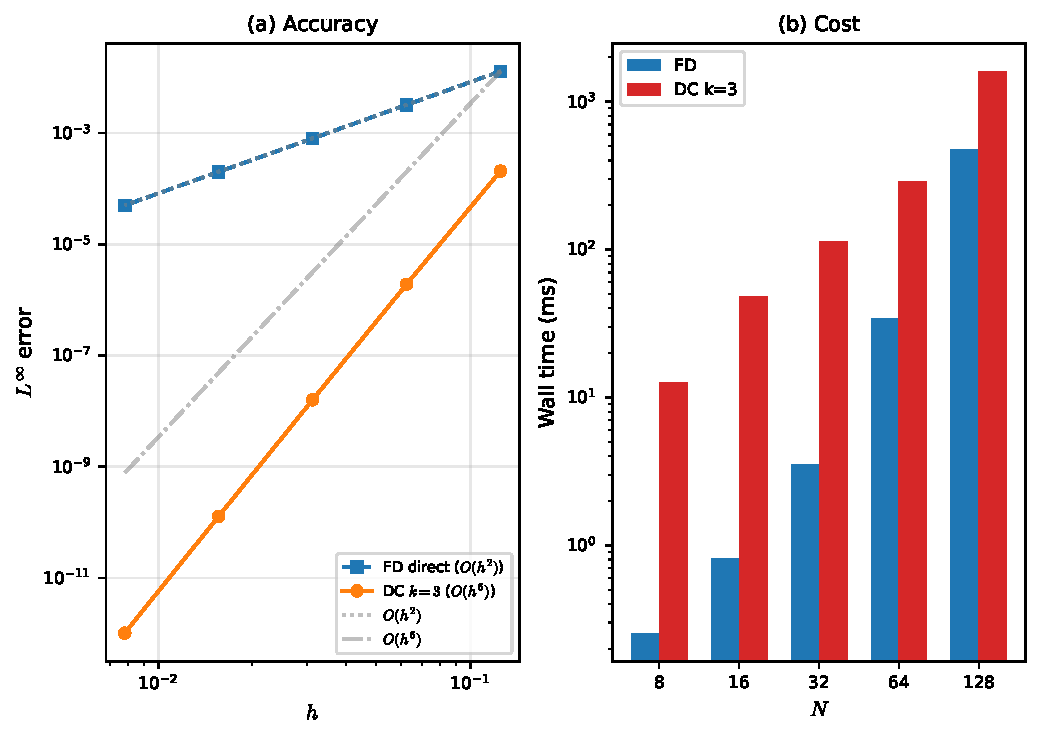
\includegraphics[width=0.72\linewidth]{figures/ch11_dc_vs_fd}
\caption{DC $k{=}3$ と FD 5 点直接解法の $L^\infty$ 誤差・計算コスト比較．
  DC は $N=128$ で FD の約 $4.9 \times 10^7$ 倍高精度でありながら，
  コスト増加は $3.4$ 倍にとどまる．}
\label{fig:dc_vs_fd}
\end{figure}

DC $k=3$ は $N = 128$ において FD の約 4900 万倍の精度を達成しつつ，
計算コストの増加は 3.4 倍にとどまる．
なお，本テストは非周期 Dirichlet 境界条件を用いているため，
§~\ref{sec:verify_ccd_convergence} の周期境界テストでは検証されなかった
CCD 境界スキームの正当性も同時に確認している．

欠陥補正法は $k=3$ で CCD の設計精度を発現させる．
次にこの反復ソルバの緩和パラメタ $\omega$ と密度比の関係を解析する．


% ─────────────────────────────────────────────────────────────────────────────
\subsubsection{DC 反復の$\omega$緩和とスペクトル収束}
\label{sec:verify_dc_spectral}
% ─────────────────────────────────────────────────────────────────────────────

前項では等密度・Dirichlet 条件で DC の精度特性を確認した．
しかし二相流シミュレーションでは密度比 $\rho_l / \rho_g$ が大きく，
DC の Step~2 におけるソルバ選択と緩和パラメタ $\omega$ が収束性を左右する．
本項では Appendix~\ref{app:dc_convergence_theory} の理論解析を数値的に裏付ける
2 つの実験を報告する．

\paragraph{(a) Thomas ADI スイープの収束限界}
2 次元 PPE（Neumann 境界，$p^* = \cos(\pi x)\cos(\pi y)$，$N = 32, 64$）に対し，
DC の Step~2 を Thomas ADI 方向分離スイープで求解した．
結果は，\textbf{すべての条件で反復が発散}した．
2 次元 ADI の反復行列の滑らかモード $(k_x, k_y) = (\pi/N, \pi/N)$ における固有値は
%
\begin{equation}
  \mu_{\mathrm{ADI}}
    \approx 1 + \lambda_{HL} \,\Delta\tau^2
    = 1 + \Ord{h^4}
\end{equation}
%
と見積もられる（$\lambda_{HL}$ は $L_H - L_L$ の滑らかモード固有値）．
$|\mu_{\mathrm{ADI}}| < 1$ を達成するには
$\Ord{N^4}$ 回（$N=32$ で $\sim 10^6$ 回）の反復が必要となる．
したがって ADI 方向分離は 2 次元 PPE の DC Step~2 ソルバとしては実用性を欠く．
なお，この発散は仮想時間反復そのものの限界ではなく，
2 次元演算子を 1 次元スイープに分裂させる際の分裂誤差 $\Delta\tau^2 L_x L_y$
に起因する．
分裂を回避し Step~2 を直接求解する次項~(b) では，
同じ DC 反復（前処理付き Richardson 反復と等価）が $\omega < 0.833$ で収束する．

\paragraph{(b) 直接 LU 分解 ＋ $\omega$-密度比収束マップ}
Step~2 を直接 LU 分解（\texttt{spsolve}）で厳密に求解し，
緩和パラメタ $\omega \in \{0.1, 0.2, 0.3, 0.5, 0.7, 0.83\}$，
密度比 $\rho_l / \rho_g \in \{1, 2, 5, 10, 20, 50, 100, 200, 500, 1000\}$
の組み合わせで DC $k=3$ の収束性を調べた（$\mathrm{tol} = 10^{-8}$，$\mathrm{maxiter} = 150$）．
表~\ref{tab:dc_omega_map} に $N = 32$ および $N = 64$ の結果を示す．

\begin{table}[htbp]
\centering
\caption{DC $k{=}3$ の $\omega$-密度比収束マップ（$\checkmark$: 収束，\textasciitilde{}: 停滞，$\times$: 発散）}
\label{tab:dc_omega_map}
\renewcommand{\arraystretch}{1.3}
\small
\begin{tabular}{r cccccc c cccccc}
\toprule
& \multicolumn{6}{c}{$N = 32$} & & \multicolumn{6}{c}{$N = 64$} \\
\cmidrule{2-7} \cmidrule{9-14}
$\rho_l/\rho_g$ & $0.1$ & $0.2$ & $0.3$ & $0.5$ & $0.7$ & $0.83$
& & $0.1$ & $0.2$ & $0.3$ & $0.5$ & $0.7$ & $0.83$ \\
\midrule
    1 & \textasciitilde{} & $\checkmark$ & $\checkmark$ & $\checkmark$ & $\checkmark$ & \textasciitilde{}
      & & \textasciitilde{} & $\checkmark$ & $\checkmark$ & $\checkmark$ & $\checkmark$ & \textasciitilde{} \\
    2 & \textasciitilde{} & \textasciitilde{} & \textasciitilde{} & \textasciitilde{} & \textasciitilde{} & \textasciitilde{}
      & & \textasciitilde{} & \textasciitilde{} & $\checkmark$ & $\checkmark$ & $\checkmark$ & \textasciitilde{} \\
$\ge 5$ & \textasciitilde{} & \textasciitilde{} & \textasciitilde{} & \textasciitilde{} & \textasciitilde{} & \textasciitilde{}
      & & \textasciitilde{} & \textasciitilde{} & \textasciitilde{} & \textasciitilde{} & \textasciitilde{} & \textasciitilde{} \\
\bottomrule
\end{tabular}
\end{table}

\begin{figure}[htbp]
\centering
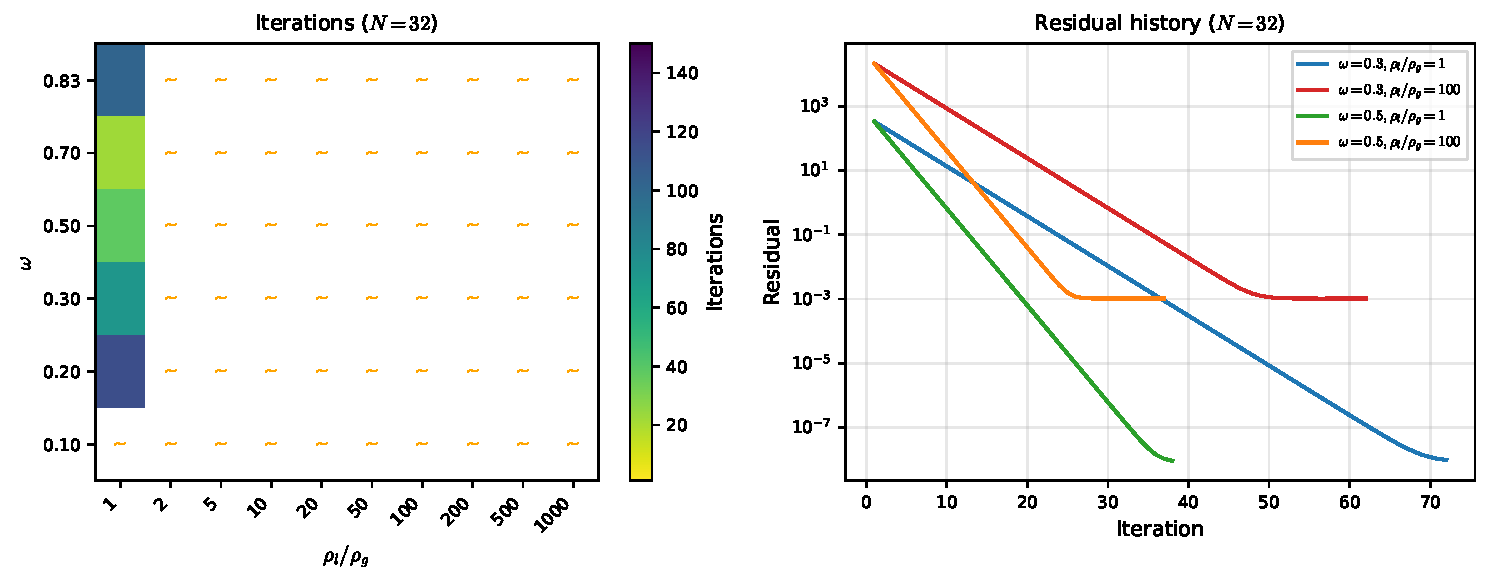
\includegraphics[width=0.48\linewidth]{figures/ch11_dc_omega_map_N32}%
\hfill
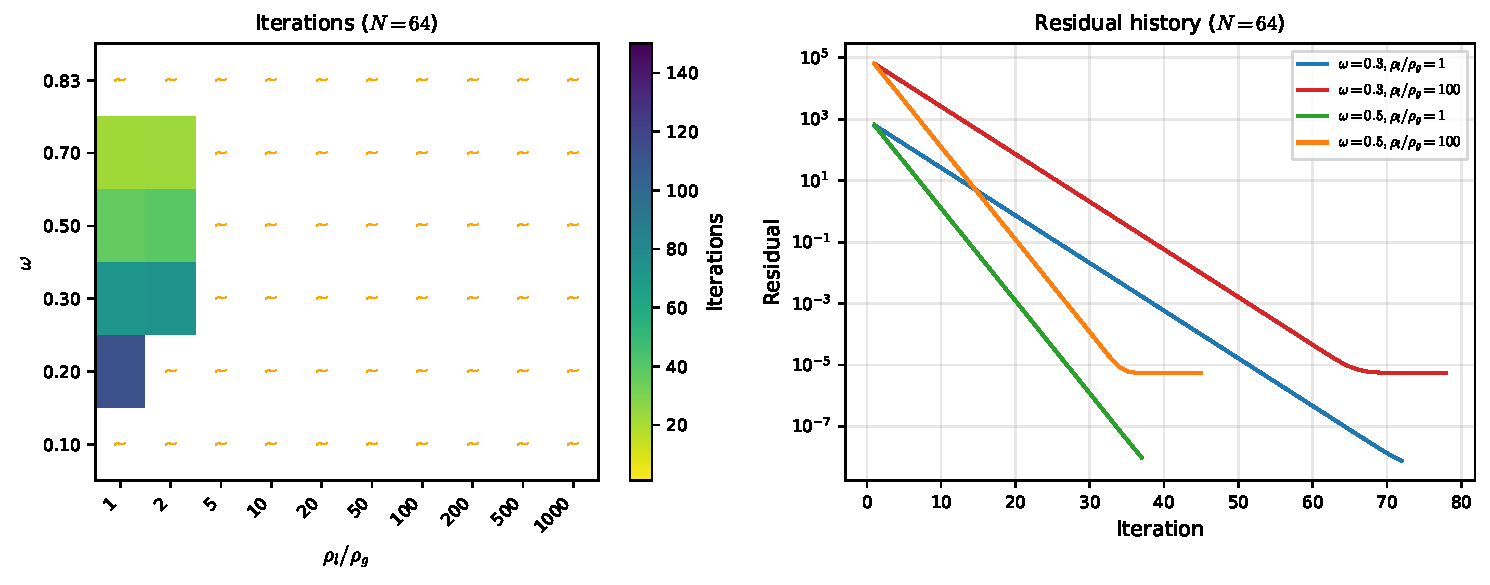
\includegraphics[width=0.48\linewidth]{figures/ch11_dc_omega_map_N64}
\caption{DC $k{=}3$ の $\omega$-密度比収束マップ．左: $N=32$，右: $N=64$．
  $\rho_l/\rho_g = 1$ では $\omega \in [0.2, 0.7]$ で収束するが，
  密度比の増加とともに収束領域が縮小する．}
\label{fig:dc_omega_map}
\end{figure}

$\rho_l/\rho_g = 1$ では $\omega \in [0.2, 0.7]$ の広い範囲で 22--115 回の反復で収束する．
$\omega = 0.83$ で停滞が生じるのは，Nyquist モードの減衰率が
$\sim 0.992 \approx 1$ となるためであり，
Appendix~\ref{app:dc_convergence_theory} が示す理論上限 $\omega_{\max} = 5/6 \approx 0.833$ と整合する．
$\rho_l/\rho_g = 2$，$N = 64$ では $\omega \in [0.3, 0.7]$ でなお収束するが，
界面幅が $3h$ 程度に狭まるため収束マージンが減少している．
$\rho_l/\rho_g \ge 5$ ではすべての $\omega$ で停滞する．
これは CCD（$\Ord{h^6}$）と FD（$\Ord{h^2}$）の密度勾配 $\bnabla\rho$ 評価差が
界面近傍で $(\rho_l/\rho_g) \cdot h^2$ に比例する残差床を形成するためであり，
高密度比条件では Krylov ソルバ（GMRES ＋ FD 前処理）への切り替えが必要となる．

DC ソルバの収束領域と密度比依存の限界を確認した．
次に，実際の PPE 境界条件である全周 Neumann 条件での精度を検証する．


% ─────────────────────────────────────────────────────────────────────────────
\subsubsection{PPE Neumann 境界条件とゲージ固定}
\label{sec:verify_ppe_neumann}
% ─────────────────────────────────────────────────────────────────────────────

§~\ref{sec:ppe_bc_stability} で議論したように，
PPE は全周 Neumann 境界条件の下で解の一意性を欠くため，
1 点ゲージ固定 $p_{0,0} = p^*(0,0)$ による拘束が不可欠である．
本項では，参照解 $p^* = \cos(\pi x)\cos(\pi y)$
（境界上で自然に $\partial p^*/\partial n = 0$ を満たす）を用い，
全周 Neumann BC ＋ゲージ固定 $p_{0,0} = p^*(0,0) = 1$ の条件で
DC $k=3$ の格子収束性を検証する．

\begin{table}[htbp]
\centering
\caption{PPE Neumann 境界条件（$p^* = \cos\pi x\,\cos\pi y$，DC $k{=}3$，ゲージ固定 $p_{0,0}=1$）}
\label{tab:ppe_neumann}
\renewcommand{\arraystretch}{1.3}
\begin{tabular}{rr cc}
\toprule
$N$ & $h$ & $L^\infty$ 誤差 & 次数 \\
\midrule
  8 & $1/8$   & $1.98 \times 10^{-2}$ & ---   \\
 16 & $1/16$  & $8.59 \times 10^{-4}$ & $4.5$ \\
 32 & $1/32$  & $2.87 \times 10^{-5}$ & $4.9$ \\
 64 & $1/64$  & $9.09 \times 10^{-7}$ & $5.0$ \\
128 & $1/128$ & $2.85 \times 10^{-8}$ & $5.0$ \\
\bottomrule
\end{tabular}
\end{table}

\begin{figure}[htbp]
\centering
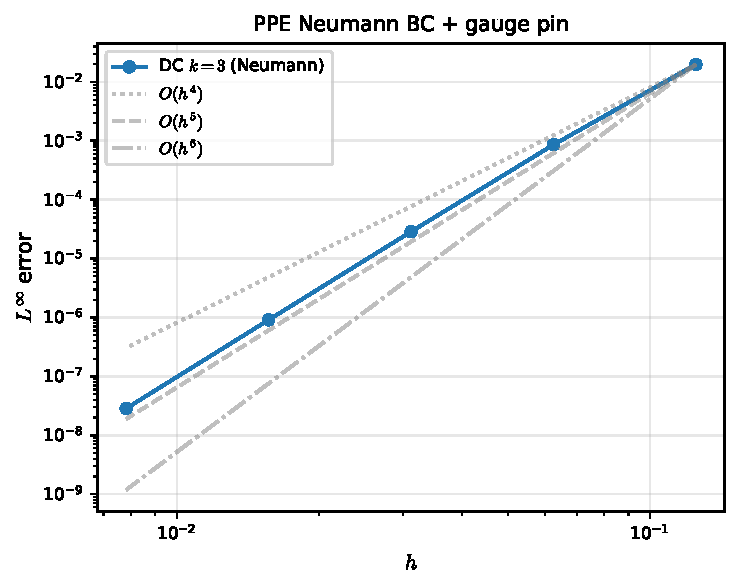
\includegraphics[width=0.72\linewidth]{figures/ch11_ppe_neumann}
\caption{PPE Neumann BC の格子収束．収束次数は $\Ord{h^5}$ に収束し，
  CCD 境界スキームの打ち切り誤差が精度上界を規定する．}
\label{fig:ppe_neumann}
\end{figure}

収束次数は $N \ge 32$ で $\Ord{h^{5.0}}$ に安定する．
これは CCD の内部スキーム（$\Ord{h^6}$）ではなく，
境界スキーム（$\Ord{h^5}$）が全体精度のボトルネックとなることを意味する．
前項 §~\ref{sec:verify_ppe} の Dirichlet テストでは
参照解が境界上で零となるため境界スキーム誤差が消失し超収束（$\Ord{h^7}$）を示したが，
Neumann 条件ではこの特殊事情がなく，境界精度が支配的となる．
二相流 PPE は Neumann 条件で運用するため，
達成可能な空間精度は $\Ord{h^5}$ が実質的な上界である．

Neumann BC では CCD 境界スキーム $\Ord{h^5}$ が精度の上界となる．
最後に，二相流で不可避となる変密度条件下の PPE 収束性を検証する．


% ─────────────────────────────────────────────────────────────────────────────
\subsubsection{変密度 PPE の収束特性と限界}
\label{sec:verify_ppe_varrho}
% ─────────────────────────────────────────────────────────────────────────────

二相流の PPE は $\bnabla \cdot (1/\rho)\,\bnabla p = f$ の形をとり，
密度 $\rho$ の空間変動が離散化精度に影響する．
§~\ref{sec:ccd_2d_full} で導出した積の法則
（式~\eqref{eq:varrho_product_rule}）を用いた DC $k=3$ ソルバの精度を，
密度比を系統的に変化させて検証する．

\paragraph{(a) 滑らかな密度場}
密度場 $\rho(x,y) = 1 + A\sin(\pi x)\cos(\pi y)$ を
$A = 0, 0.8, 0.98, 0.998$（$\rho_{\max}/\rho_{\min} \approx 1, 9, 99, 999$）
の 4 水準で設定し，
$p^* = \sin(\pi x)\sin(\pi y)$（Dirichlet BC），DC $k=3$，$N = 16, 32, 64, 128$
で格子収束試験を行った．

\begin{table}[htbp]
\centering
\caption{変密度 PPE の格子収束（滑らかな密度場，DC $k{=}3$，Dirichlet BC）}
\label{tab:varrho_ppe}
\renewcommand{\arraystretch}{1.3}
\begin{tabular}{r cccc}
\toprule
$N$ & $\rho_{\max}/\rho_{\min} \approx 1$ & $\approx 9$ & $\approx 99$ & $\approx 999$ \\
\midrule
 16 & $1.91 \times 10^{-6}$  & $2.06 \times 10^{-6}$  & $3.12 \times 10^{-6}$  & $7.79 \times 10^{-6}$  \\
 32 & $1.60 \times 10^{-8}$  & $1.74 \times 10^{-8}$  & $7.32 \times 10^{-8}$  & $2.67 \times 10^{-7}$  \\
 64 & $1.29 \times 10^{-10}$ & $1.41 \times 10^{-10}$ & $8.47 \times 10^{-10}$ & $4.76 \times 10^{-9}$  \\
128 & $1.02 \times 10^{-12}$ & $1.51 \times 10^{-12}$ & $1.82 \times 10^{-11}$ & $8.50 \times 10^{-11}$ \\
\midrule
\multicolumn{1}{c}{次数$^*$} & $\approx 7.0$ & $\approx 6.5$ & $\approx 5.5$ & $\approx 5.8$ \\
\bottomrule
\multicolumn{5}{l}{\footnotesize $^*$ $N=64{\to}128$ のペアによる漸近値．高密度比では前漸近領域で次数が振動する．} \\
\end{tabular}
\end{table}

\begin{figure}[htbp]
\centering
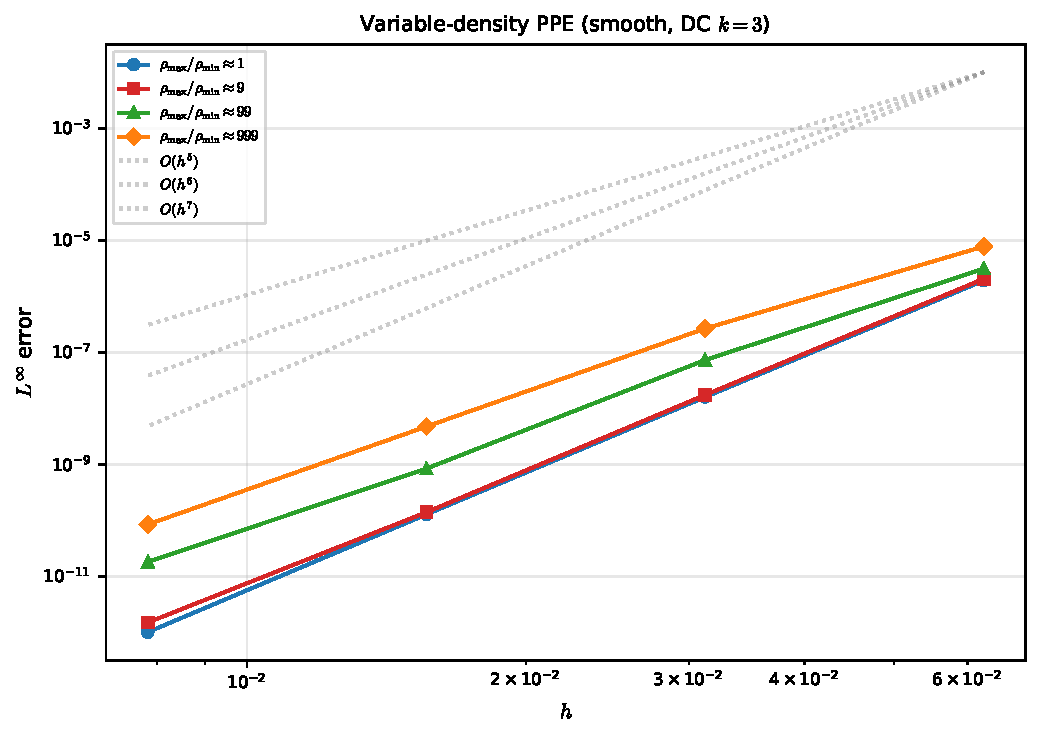
\includegraphics[width=0.72\linewidth]{figures/ch11_varrho_ppe}
\caption{変密度 PPE の格子収束（滑らかな密度場）．
  密度比 $\rho_{\max}/\rho_{\min} \approx 999$ でも $\Ord{h^{5.8}}$ を維持する．}
\label{fig:varrho_ppe}
\end{figure}

等密度（$A=0$）の結果は §~\ref{sec:verify_ppe} の Dirichlet テストと一致し $\Ord{h^7}$ を再現する．
$\rho_{\max}/\rho_{\min} \approx 999$ においても漸近収束次数は $\Ord{h^{5.8}}$ を維持し，
$N=128$ で $L^\infty = \Ord{10^{-11}}$ を達成した．
密度場が十分に滑らかである限り，CCD の高次精度は密度比によらず発現する．

\paragraph{(b) 界面型密度分布（平滑化 Heaviside）—— 収束の破綻}
\label{sec:varrho_ppe_limitation}

実際の二相流では界面を挟んで密度が急峻に変化する．
平滑化 Heaviside 関数による界面型密度分布
（$\rho_l/\rho_g = 10, 100, 1000$）を設定し，
$N=64$，DC $k=3$ で求解を試みた．

\begin{table}[htbp]
\centering
\caption{界面型密度分布での PPE 求解（平滑化 Heaviside，$N=64$，DC $k{=}3$）}
\label{tab:varrho_ppe_interface}
\renewcommand{\arraystretch}{1.3}
\begin{tabular}{r c l}
\toprule
$\rho_l/\rho_g$ & $L^\infty$ 誤差 & 状態 \\
\midrule
    1 & $1.3 \times 10^{-10}$ & 収束（$\Ord{h^7}$） \\
   10 & $1.3$                 & 非収束（振動） \\
  100 & $1.1 \times 10^{5}$   & 発散 \\
 1000 & $3.7 \times 10^{3}$   & 発散 \\
\bottomrule
\end{tabular}
\end{table}

$\rho_l/\rho_g \ge 10$ で解が破綻する．
根本原因は，$1/\rho$ が界面を挟んで $\rho_l/\rho_g$ 倍のジャンプを持つことにある．
界面を横断するステンシル（FD・CCD を問わず）は $\Ord{1}$ の離散化誤差を生じ，
結果として反復行列 $L_L^{-1}L_H$ のスペクトル半径が 1 を超え反復が発散する．
これは平滑化 Heaviside による密度分布の一括求解に固有の本質的限界であり，
§~\ref{sec:ppe_condition_number} の条件数解析が予測する挙動と一致する．

解決策として，分相 PPE（phase-split PPE）——各相で等密度の PPE を独立に解き，
$[p] = \sigma\kappa$ の圧力跳びを HFE で界面条件として課す方式——が考えられる．
この方式であれば界面横断ステンシルが排除され，
各相内で §~\ref{sec:verify_ppe} の等密度精度が回復する．

以上で PPE ソルバの空間精度と限界を確認した．
次節では，アルゴリズム Step~1（CLS 移流）と Step~5（Predictor）で用いる
2 つの時間積分スキームの精度を検証する．
                %% §11.3 圧力ソルバの検証
% paper/sections/11_time.tex
%
% §11.4  時間積分スキームの検証
%   Exp 14: TVD-RK3
%   Exp 15: AB2
% ═══════════════════════════════════════════════════════════════════════════════

\subsection{時間積分スキームの検証}
\label{sec:verify_time}

前節では PPE ソルバの空間精度と収束特性を検証した．
本節では，アルゴリズム Step~1（CLS 移流）で用いる TVD-RK3
（§\ref{sec:verify_tvd_rk3}）と
Step~5（Predictor）で用いる AB2（§\ref{sec:verify_ab2}）の
時間積分精度を確認する．


% ─────────────────────────────────────────────────────────────────────────────
\subsubsection{TVD-RK3 時間積分精度}
\label{sec:verify_tvd_rk3}
% ─────────────────────────────────────────────────────────────────────────────

\noindent\textbf{目的：}
§~\ref{sec:time_int} で導入した TVD-RK3（3 段 Shu--Osher 型 Runge--Kutta）の
設計時間精度 $\Ord{\Delta t^3}$ をスカラー ODE テストで確認する．

\noindent\textbf{評価対象：}
TVD-RK3（3 段 Shu--Osher 型 Runge--Kutta）．

\noindent\textbf{手順とパラメタ：}
\begin{itemize}[noitemsep]
  \item スカラー ODE $\mathrm{d}q/\mathrm{d}t = -q$，$q(0)=1$，厳密解 $q(1) = e^{-1}$
  \item ステップ数 $n = 16, 32, 64, 128, 256, 512$
\end{itemize}

\noindent\textbf{結果：}

\begin{table}[htbp]
\centering
\caption{TVD-RK3 の時間精度（$\mathrm{d}q/\mathrm{d}t=-q$，$q(0)=1$）}
\label{tab:tvd_rk3}
\renewcommand{\arraystretch}{1.3}
\begin{tabular}{rc cc}
\toprule
$n$ & $\Delta t$ & $|q - e^{-1}|$ & 次数 \\
\midrule
 16 & $6.25 \times 10^{-2}$ & $3.55 \times 10^{-5}$  & ---    \\
 32 & $3.13 \times 10^{-2}$ & $4.39 \times 10^{-6}$  & $3.02$ \\
 64 & $1.56 \times 10^{-2}$ & $5.46 \times 10^{-7}$  & $3.01$ \\
128 & $7.81 \times 10^{-3}$ & $6.81 \times 10^{-8}$  & $3.00$ \\
256 & $3.91 \times 10^{-3}$ & $8.51 \times 10^{-9}$  & $3.00$ \\
512 & $1.95 \times 10^{-3}$ & $1.06 \times 10^{-9}$  & $3.00$ \\
\bottomrule
\end{tabular}
\end{table}

\begin{figure}[htbp]
\centering
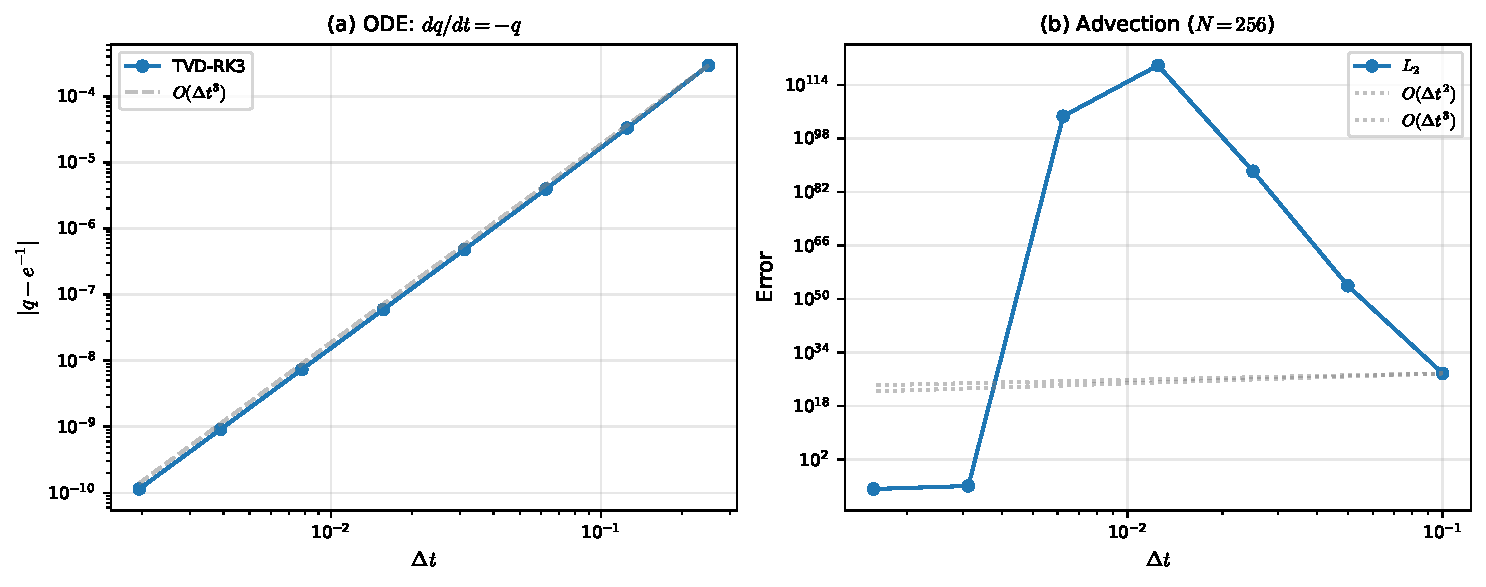
\includegraphics[width=0.72\linewidth]{figures/ch11_tvd_rk3}
\caption{TVD-RK3 の時間収束．設計通り $\Ord{\Delta t^3}$ の 3 次精度を達成する．}
\label{fig:tvd_rk3}
\end{figure}

\noindent\textbf{結論：}
収束次数はすべての格子幅で $3.00$--$3.02$ を示し，設計通りの $\Ord{\Delta t^3}$ が確認された．


% ─────────────────────────────────────────────────────────────────────────────
\subsubsection{AB2 時間積分精度}
\label{sec:verify_ab2}
% ─────────────────────────────────────────────────────────────────────────────

\noindent\textbf{目的：}
§~\ref{sec:ab2_ipc} で導入した AB2（Adams--Bashforth 2 段）の
設計時間精度 $\Ord{\Delta t^2}$ を確認する．

\noindent\textbf{評価対象：}
AB2（Adams--Bashforth 2 段）＋前進 Euler 起動．

\noindent\textbf{手順とパラメタ：}
\begin{itemize}[noitemsep]
  \item スカラー ODE $\mathrm{d}q/\mathrm{d}t = -q$，$q(0)=1$，厳密解 $q(1) = e^{-1}$
  \item 初期ステップは前進 Euler で起動
  \item ステップ数 $n = 16, 32, 64, 128, 256, 512$
\end{itemize}

\noindent\textbf{結果：}

\begin{table}[htbp]
\centering
\caption{AB2 の時間精度（$\mathrm{d}q/\mathrm{d}t=-q$，$q(0)=1$，初期ステップ: 前進 Euler）}
\label{tab:ab2_time}
\renewcommand{\arraystretch}{1.3}
\begin{tabular}{rc cc}
\toprule
$n$ & $\Delta t$ & $|q - e^{-1}|$ & 次数 \\
\midrule
 16 & $6.25 \times 10^{-2}$ & $1.42 \times 10^{-4}$ & ---    \\
 32 & $3.13 \times 10^{-2}$ & $3.27 \times 10^{-5}$ & $2.12$ \\
 64 & $1.56 \times 10^{-2}$ & $7.84 \times 10^{-6}$ & $2.06$ \\
128 & $7.81 \times 10^{-3}$ & $1.92 \times 10^{-6}$ & $2.03$ \\
256 & $3.91 \times 10^{-3}$ & $4.73 \times 10^{-7}$ & $2.02$ \\
512 & $1.95 \times 10^{-3}$ & $1.18 \times 10^{-7}$ & $2.01$ \\
\bottomrule
\end{tabular}
\end{table}

\begin{figure}[htbp]
\centering
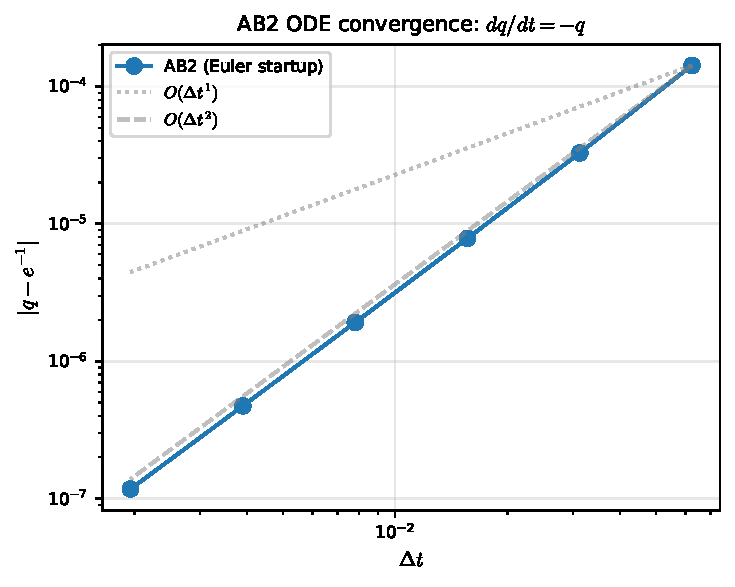
\includegraphics[width=0.72\linewidth]{figures/ch11_ab2_time}
\caption{AB2 の時間収束．寄生根 $|\rho_2| = 0.5$ により Euler 起動の
  $\Ord{\Delta t}$ 誤差は数ステップで減衰し，全体として $\Ord{\Delta t^2}$ を達成する．}
\label{fig:ab2_time}
\end{figure}

\noindent\textbf{結論：}
収束次数は $\Ord{\Delta t^2}$ に漸近し，設計通りの 2 次精度が確認された．
AB2 の特性方程式が持つ寄生根 $|\rho_2| = 0.5$ は安定領域内にあり，
前進 Euler による $\Ord{\Delta t}$ の起動誤差は数ステップで減衰する．

以上で全 17 コンポーネントの単体検証が完了した．次節に結果を総括する．
                  %% §11.4 時間積分スキームの検証
\input{sections/11_summary}               %% §11.5 検証結果の総括
